\documentclass{beamer}
%
% Choose how your presentation looks.
%
% For more themes, color themes and font themes, see:
% http://deic.uab.es/~iblanes/beamer_gallery/index_by_theme.html
%
\mode<presentation>
{
  \usetheme{default}      % or try Darmstadt, Madrid, Warsaw, ...
  \usecolortheme{crane} % or try albatross, beaver, crane, ...
  \usefonttheme{structureitalicserif}  % or try serif, structurebold, ...
  \setbeamertemplate{navigation symbols}{}
  \setbeamertemplate{caption}[numbered]
} 

\usepackage[english]{babel}
%\usepackage[utf8x]{inputenc}
\usepackage{mathrsfs}

\newtheorem{proposition}{Proposition}
\newtheorem{rem}{Remark}
\newtheorem{goal}{Goal}
\newtheorem{Conjecture}{Conjecture}

\title[Artin Group Presentations]{Artin Group Presentations Arising from Cluster Algebras}
\author{Jacob Haley*, David Hemminger, Aaron Landesman, 
Hailee Peck*}
\institute{University of Minnesota, Twin Cities REU}
\date{\today}


\begin{document}

\begin{frame}
  \titlepage
  \let\thefootnote\relax\footnote{* denotes speaker}
\end{frame}

 
\begin{frame}{Outline}
  \tableofcontents
\end{frame}

\begin{frame}{Brief History}
Fomin and Zelevinsky introduced \textit{cluster algebras}, generated from seed variables. These algebras are of finite type if they are generated from a finite number of cluster variables. Fomin and Zelevinsky also showed that cluster algebras of finite type can be classified by Dynkin diagrams.
\begin{figure}
\centering
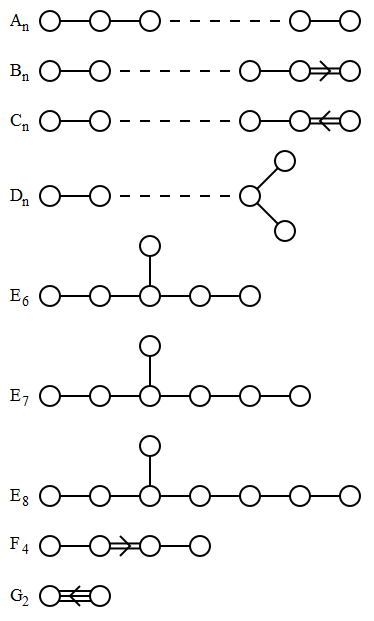
\includegraphics[scale = .25]{dynkindiagrams.PNG}
\caption{Dynkin diagrams}
\end{figure}
\end{frame}

\begin{frame}{Example}
\begin{figure}
\centering
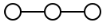
\includegraphics[scale = .65]{DynkinA3.PNG}
\caption{Dynkin diagram of type $A_3$}
\end{figure}

Coxeter group relations:
\begin{itemize}
\item $s_i^2 = e$ :  $s_1^2 = s_2^2 = s_3^2 = e$ 
\item $(s_is_j)^{m_{ij}} = e$ :  $(s_1s_2)^3 = (s_2s_3)^3 = e$
\item  $(s_is_j)^{m_{ij}} = e$ :  $(s_1s_3)^2 = e$
\end{itemize}

Artin group relations:
\begin{itemize}
\item $s_1s_2s_1 = s_2s_1s_2$
\item $s_2s_3s_2 = s_3s_2s_3$
\item $s_1s_3 = s_3s_1$
\end{itemize}

\end{frame}


\begin{frame}
Barot and Marsh extended the Coxeter group presentations to diagrams of finite type (making an allowance for chordless cycles).
\begin{theorem}
[Theorem 5.4, Barot-Marsh]
\begin{enumerate}
\item Let $\Gamma$ be a diagram of finite type and $\Gamma^{\prime} = \mu_k(\Gamma)$ the mutation of $\Gamma$ at vertex $k$. Then $W_{\Gamma} \cong W_{\Gamma^{\prime}}$.
\item Let $\mathscr{A}$ be a cluster algebra of finite type. Then the groups $W_{\Gamma}$ associated to the diagrams $\Gamma$ arising from the seeds of $\mathscr{A}$ are all isomorphic (to the reflection group associated to the Dynkin diagram associated to $\mathscr{A}$).
\end{enumerate}
\end{theorem}


\pause
\begin{theorem}{(HHLP, 14)}
 Let $\Gamma$ be a diagram of finite type and $\Gamma^{\prime} = \mu_k(\Gamma)$ the mutation of $\Gamma$ at vertex $k$. Then $A_{\Gamma} \cong A_{\Gamma^{\prime}}$. 
\end{theorem}
\end{frame}

\section{Preliminary Definitions}

\begin{frame}
\begin{definition}
We say a matrix $B$ is \textit{skew-symmetrisable} if there exists a diagonal matrix $D$ of the same size such that $D_{ii}>0$ and $DB$ is skew-symmetric.
\end{definition}

\pause

\begin{definition}
A skew-symmetrisable matrix $B$ is \textit{2-finite} if $|B_{ij}B_{ji}| \leq 3$ for all $i, j \in \{ 1, \ldots, n \}$.
\end{definition}

\pause

From the skew-symmetrisable matrix associated to a cluster algebra of finite type, we can associate an diagram $\Gamma$ as follows:\\


For $i, j \in V(\Gamma)$, $i \xrightarrow{w} j$ if and only if $B_{ij}>0$ and $w = |B_{ij}B_{ji}|$ is the weight of the edge.

\end{frame}


\section{Background Results}

\subsection{Mutation Rules}

\begin{frame}{Mutation Rules}
\begin{proposition}
[Proposition 1.4, Barot-Marsh]
Let $B$ be a $2$-finite skew-symmetrisable matrix. Then $\Gamma(\mu_k(B))$ is uniquely determined by $\Gamma(B)$ as follows:
\begin{itemize}
\item Reverse the orientations of all edges in $\Gamma(B)$ incident with $k$ (leaving the weights unchanged)
\item For any path in $\Gamma(B)$ of form $i \xrightarrow{a} k \xrightarrow{b} j$ (i.e. with $a,b$ positive), let $c$ be the weight on the edge $j \rightarrow i$, taken to be zero if there is no such arrow. Let $c'$ be determined by $c'\geq 0$ and 
$c+c' =$ max$(a,b)$. 
Then $\Gamma(B)$ changes in a predetermined way, taking the case $c' = 0$ to mean no arrow between $i$ and $j$.

%%SHOW THE PREDETERMINED WAY ON THE BOARD
\end{itemize}
\end{proposition}

\end{frame}

\begin{frame}{Mutation Rules}
\begin{figure}[h]
\centering
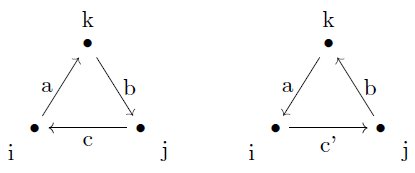
\includegraphics[scale = .65]{mutationrules.PNG}
\caption{Predetermined method for mutation at $k$}
\end{figure}
\end{frame}

\subsection{Chordless cycles underlying $\Gamma$}

\begin{frame}{Unoriented structures underlying $\Gamma$}
\begin{proposition}
[Proposition 9.7, Fomin-Zelevinsky II]
Any chordless cycle in $\Gamma$ must have an unoriented structure that is one of the following. Furthermore, it must be cyclically oriented.
\begin{figure}[h]
\centering
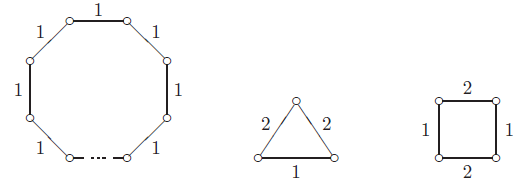
\includegraphics[scale = .65]{chordlesscycles.PNG}
\caption{Possible chordless cycles in a diagram}
\end{figure}

\end{proposition}
\end{frame}

\begin{frame}
\tableofcontents 
\end{frame}

\section{Coxeter group presentation (Barot-Marsh)}

\begin{frame}{Coxeter group presentation}
\begin{definition}
For a diagram $\Gamma$ and $i, j \in V(\Gamma)$, define 
\begin{displaymath}
m_{ij} = \begin{cases}    2 & \mbox{if } i \mbox{ and } j \mbox{ are not connected;} \\
						3 & \mbox{if } i \mbox{ and } j \mbox{ are connected by an edge of weight } 1;\\
						4 & \mbox{if } i \mbox{ and } j \mbox{ are connected by an edge of weight } 2;\\
						6 & \mbox{if } i \mbox{ and } j \mbox{ are connected by an edge of weight } 3.\\
					\end{cases}
\end{displaymath}	
\end{definition}

This definition will allow us to present generator relations in the group $W_{\Gamma}$.
\end{frame}

\subsection{Generators and Relations}

\begin{frame}{Coxeter group presentation}

Given a diagram $\Gamma$ of finite type, Barot and Marsh define the Coxeter group $W_{\Gamma}$ with generators $s_i, i = 1,2,\ldots, n$, subject to the following relations:
\begin{block}
   
\begin{itemize}
\item{\alert{(R1)}} $s_i^2 = e$ for all $i$
\item{\alert{(R2)}} $\left(s_is_j\right)^{m_{ij}} = e$ for all $i \neq j$
\end{itemize}

Furthermore, for a chordless cycle $C : i_0 \rightarrow i_1 \rightarrow \cdots \rightarrow i_{d-1} \rightarrow i_0$ and for $a = 0,1,2,\ldots, d-1$, define \textbf{$r\left(i_a, i_{a+1}\right) = s_{i_a}s_{i_{a+1}} \cdots s_{i_{a+d-1}}s_{i_{a+d-2}} \cdots s_{i_{a+1}}$}.\\

\vspace{0.1cm}
Then we have the following relations:
\begin{itemize}
\item{\alert{(R3)(a)}} If all the weights in the edges of $C$ are $1$, then $r(i_a, i_{a+1})^2 = e$
\item{\alert{(R3)(b)}} If $C$ has some edges of weight $2$, then $r(i_a, i_{a+1})^k = e$ where $k = 4-w_a$ and $w_a$ is the weight of the edge $i_a\--\ i_{a-1}$
\end{itemize}
\end{block}
\end{frame}


\subsection{Invariance under Mutation Equivalence}

\begin{frame}{Coxeter group invariance}
Given a diagram $\Gamma$ and the corresponding Coxeter group $W_{\Gamma}$, Barot and Marsh prove that this group is invariant (up to isomorphism) under mutation of $\Gamma$.

\begin{theorem}
[Theorem 5.4, Barot-Marsh]
\begin{enumerate}
\item Let $\Gamma$ be a diagram of finite type and $\Gamma^{\prime} = \mu_k(\Gamma)$ the mutation of $\Gamma$ at vertex $k$. Then $W_{\Gamma} \cong W_{\Gamma^{\prime}}$.
\item Let $\mathscr{A}$ be a cluster algebra of finite type. Then the groups $W_{\Gamma}$ associated to the diagrams $\Gamma$ arising from the seeds of $\mathscr{A}$ are all isomorphic (to the reflection group associated to the Dynkin diagram associated to $\mathscr{A}$).
\end{enumerate}
\end{theorem}
\end{frame}


\section{Artin group presentation (HHLP, 14)}

\begin{frame}{Artin group presentation}
\begin{block}

Let
\begin{align*}
\langle x_i,x_j \rangle ^k = \begin{cases}
(x_ix_j)^{\frac{k}{2}}, &\text{ if }k \equiv 0 \pmod 2\\
(x_ix_j)^{\frac{k-1}{2}}x_i &\text{ if } k \equiv 1 \pmod 2
\end{cases}
\end{align*}
\end{block}

\begin{block}

Let $(i_0,\ldots, i_{d-1})$ be an ordered tuple such that the subgraph of $\Gamma$ on the vertices $i_0,\ldots, i_{d-1}$ is a chordless cycle, with edges of nonzero weight from $i_k$ to $i_{k+1}$, where subscripts are taken $\pmod d.$ Then, denote $$p(i_a,i_{a+1}) = s_{i_{a+1}}^{-1}s_{i_{a+2}}^{-1}\dots s_{i_{a-2}}^{-1}s_{i_{a-1}}s_{i_{a-2}}s_{i_{a-3}}\dots s_{i_{a+1}}.$$
\end{block}

\end{frame}
\begin{frame}{Artin group presentation}
Now we have 
\begin{align*}
\langle x_i,x_j \rangle ^k = \begin{cases}
(x_ix_j)^{\frac{k}{2}}, &\text{ if }k \equiv 0 \pmod 2\\
(x_ix_j)^{\frac{k-1}{2}}x_i &\text{ if } k \equiv 1 \pmod 2
\end{cases}
\end{align*}
And $$p(i_a,i_{a+1}) = s_{i_{a+1}}^{-1}s_{i_{a+2}}^{-1}\dots s_{i_{a-2}}^{-1}s_{i_{a-1}}s_{i_{a-2}}s_{i_{a-3}}\dots s_{i_{a+1}}.$$

Additionally, let $$t(i_a,i_{a+1}) = s_{i_a} p(i_a,i_{a+1})  s_{i_a}^{-1}p(i_a,i_{a+1})^{-1}.$$

These definitions will allow us to present generator relations in the group $A_{\Gamma}$.

\end{frame}


\subsection{Generators and Relations}

\begin{frame}{Artin group presentation}
Given a diagram $\Gamma$ of finite type, we define the Artin group $A_{\Gamma}$ with generators $s_i, i = 1,2,\ldots, n$, subject to the following relations (noting that $t(i_a,i_{a+1}) = s_{i_a} p(i_a,i_{a+1})  s_{i_a}^{-1}p(i_a,i_{a+1})^{-1}$):

\begin{block}

\begin{itemize}

\item{\alert{(T2)}} With $m_{ij}$ as defined previously, for all $i \neq j,$ we add the relations
$\langle s_i,s_j \rangle^{m_{ij}}= \langle s_j,s_i \rangle^{m_{ij}}.$

\item{\alert{(T3)}} Let $(i_0,i_1,\ldots,i_{d-1})$ be an ordered tuple as before. If additionally one of the following two conditions hold:
\begin{enumerate}
\item All edges in the chordless cycle are of weight 1 or 2 and the edge $i_{d-1}\rightarrow i_0$ has weight 2.
\item All edges in the chordless cycle have weight $1.$
\end{enumerate}
then we include the relation
$t(i_0,i_1) = e.$

\end{itemize}

\end{block}
\end{frame}

\begin{frame}{Example}
\begin{figure}
\centering
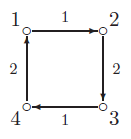
\includegraphics[scale=.5]{4cycle.PNG}
\caption{A 4 cycle with edge weights of 1 and 2}
\end{figure}

\small
Coxeter relations:
\begin{itemize}
\item[R1] $s_1^2 = s_2^2 = s_3^2 = s_4^2 = e$
\item[R2] $(s_1s_2)^3 = (s_3s_4)^3 = e$
\item[R2] $(s_2s_3)^4 = (s_4s_1)^4 = e$
\item[R2] $(s_1s_3)^2 = (s_2s_4)^2 = e$
\item[R3] $r(1,2)^2 = r(3,4)^2 = e$, or $(s_1s_2s_3s_4s_3s_2)^2 = (s_3s_4s_1s_2s_1s_4)^2 = e$
\item[R3] $r(2,3)^3 = r(4,1)^3 = e$, or $(s_2s_3s_4s_1s_4s_3)^3 = (s_4s_1s_2s_3s_2s_1)^3 = e$
\end{itemize}
\end{frame}

\begin{frame}{Example}
\begin{figure}
\centering
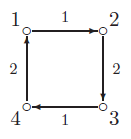
\includegraphics[scale=.5]{4cycle.PNG}
\caption{A 4 cycle with edge weights of 1 and 2}
\end{figure}

\small
Artin relations:
\begin{itemize}
\item[T2] $\langle s_1, s_2 \rangle ^3 = \langle s_2, s_1 \rangle ^3$, or $s_1s_2s_1 = s_2s_1s_2$
\item[T2] $\langle s_2, s_3 \rangle ^4 = \langle s_3, s_2 \rangle ^4$, or $s_2s_3s_2s_3 = s_3s_2s_3s_2$
\item[T2] $\langle s_2, s_4 \rangle ^2 = \langle s_4, s_2 \rangle ^2$, or $s_2s_4 = s_4s_2$
\end{itemize}
The T2 relations $\langle s_3, s_4 \rangle, \langle s_4, s_1 \rangle, \langle s_1, s_3 \rangle$ can be defined in a similar manner.
\begin{itemize}
\item[T3] $t(1,2) = s_1s_2^{-1}s_3^{-1}s_4s_3s_2s_1^{-1}s_2^{-1}s_3^{-1}s_4^{-1}s_3s_2 = e$, or $s_1s_2^{-1}s_3^{-1}s_4s_3s_2 = s_2^{-1}s_3^{-1}s_4s_3s_2s_1$.
\end{itemize}

The T3 relation $t(3,4) = e$ can be defined in a similar manner.
\end{frame}



\subsection{Invariance under Mutation Equivalence}

\begin{frame}{Artin group invariance}
Given a diagram $\Gamma$ and the corresponding Artin group $A_{\Gamma}$, we prove this group is invariant (up to isomorphism) under mutation of $\Gamma$.

\begin{theorem}{(HHLP, 14)}
Let $\Gamma$ be a diagram of finite type, and let $\Gamma^{\prime} = \mu_k(\Gamma)$ be the mutation of $\Gamma$ at vertex $k$. Then $A_{\Gamma} \cong A_{\Gamma^{\prime}}$.
\end{theorem}
\end{frame}

\section{Constructing the Isomorphism}

\begin{frame}{Constructing the Isomorphism}
To prove this theorem, our strategy will be to construct homomorphisms so that the following diagram commutes.
\begin{figure}
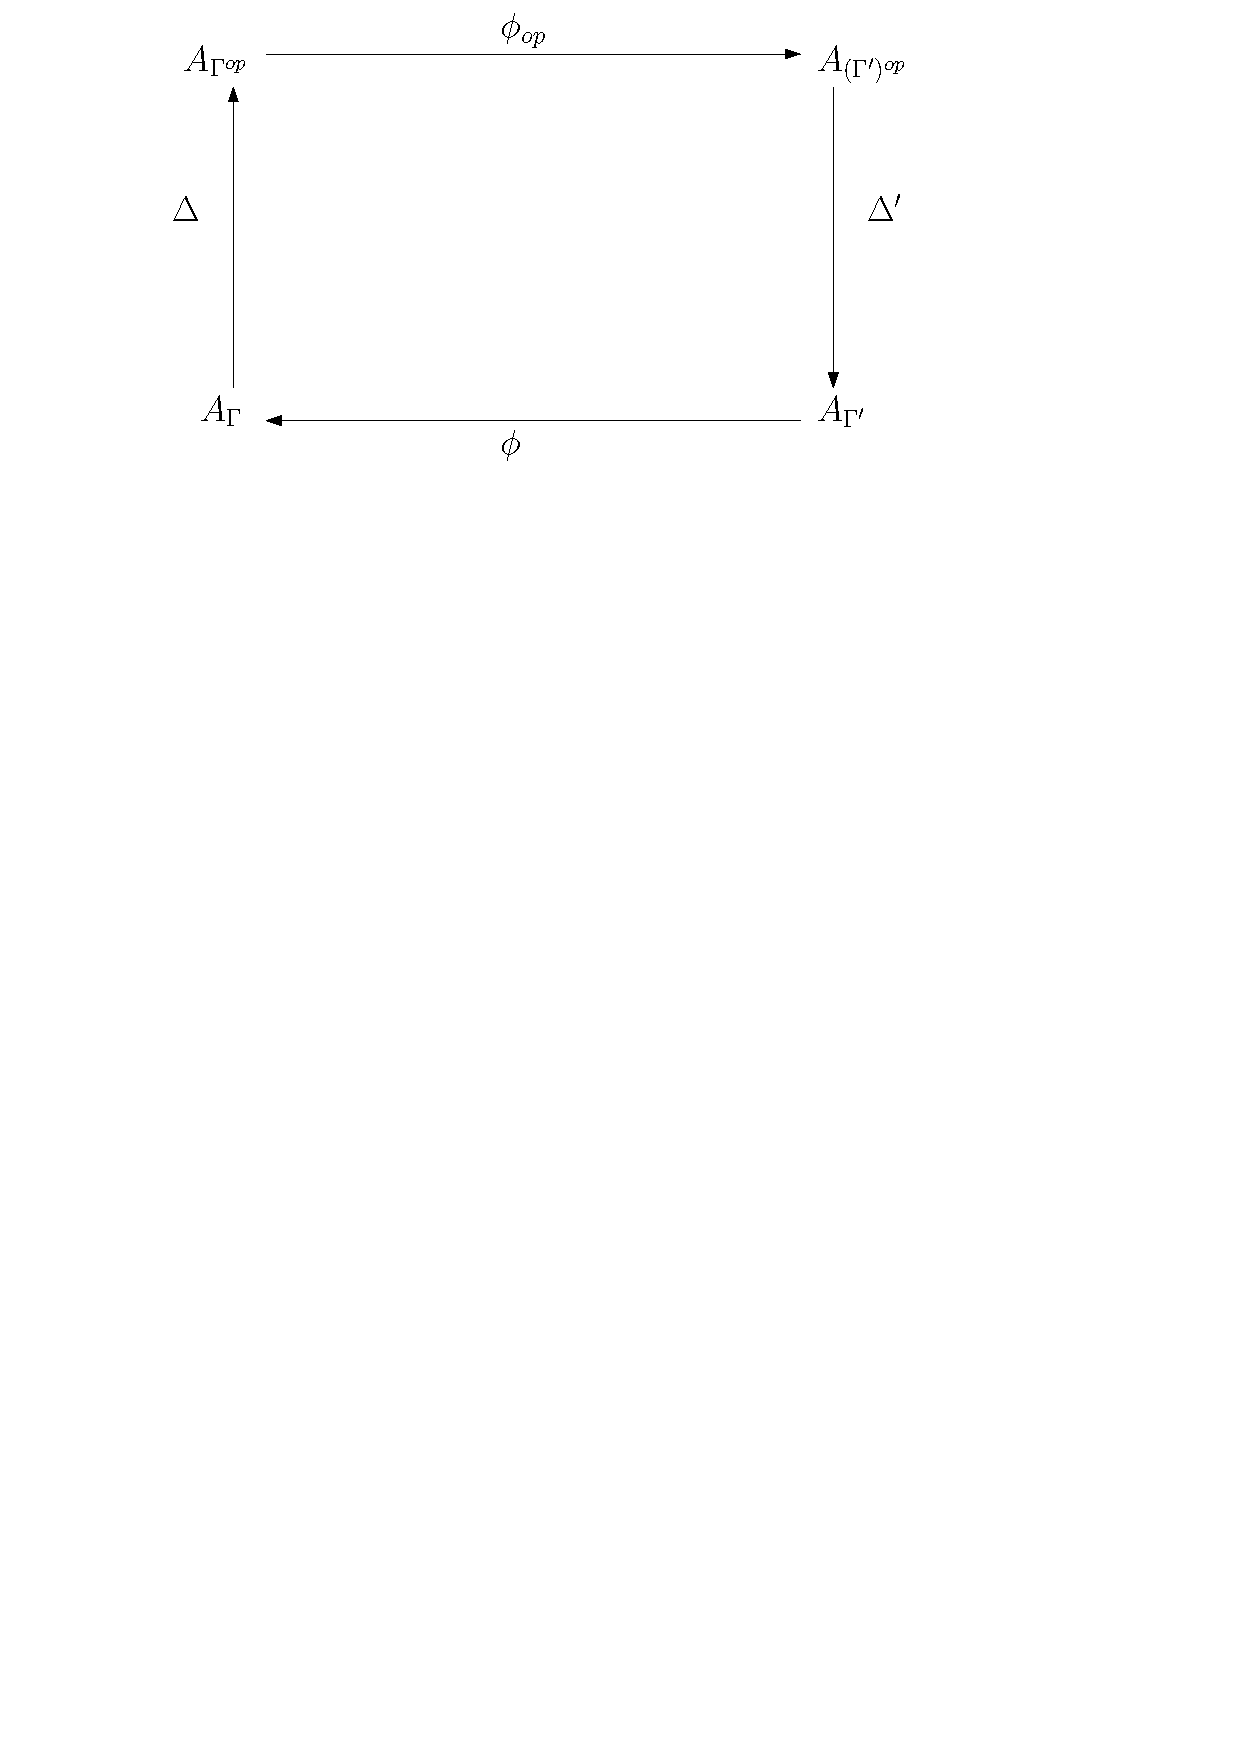
\includegraphics[scale = .50]{Comm-Diag.pdf}
\end{figure}
Then the map $\phi$ will give us the desired isomorphism.
\end{frame}

\begin{frame}{Constructing the Isomorphism}
We first prove that $A_{\Gamma} \cong A_{\Gamma^{op}}$, where $\Gamma^{op}$ is the diagram obtained by reversing all arrows in $\Gamma$.
\begin{lemma}
Let A$_{\Gamma}$ be generated by $s_{1}, \dots, s_{n}$, and let A$_{\Gamma^{op}}$ be generated by $r_{1}, \dots, r_{n}$. Then the map $$\Delta: s_{i} \rightarrow r_{i}^{-1}$$ defines an isomorphism between A$_{\Gamma}$ and A$_{\Gamma^{op}}.$
\end{lemma}
\end{frame}

\begin{frame}{Constructing the Isomorphism}
Now let $A_{\Gamma}$ be generated by $s_{1}, \dots, s_{n}$ and let $A_{\Gamma^{\prime}}$ be generated by $u_{1}, \dots, u_{n}$. Consider the map $\phi: A_{\Gamma^{\prime}} \rightarrow A_{\Gamma}$ defined as follows:
$$\phi(u_{i}) = 
\begin{cases}
s_{k}s_{i}s_{k}^{-1} &\text{if there is an arrow from i to k in $\Gamma$} \\
s_{i} &\text{otherwise}
\end{cases}$$

\begin{lemma}
The map $\phi$ is a well-defined homomomorphism.
\end{lemma}
\end{frame}

\begin{frame}{Unoriented structures underlying $\Gamma$}
In proving that the map is well-defined, we make use of the fact that diagrams of finite-type have a nice underlying structure. For example, when dealing with the (T2) relations, we have
\begin{lemma}
[Lemma 2.2, Barot-Marsh]
For $\Gamma$ of finite-type, if we have a subdiagram of $\Gamma$ with three connected vertices, then the unoriented graph underlying the subdiagram must be one of the following:
\begin{figure}[h]
\centering
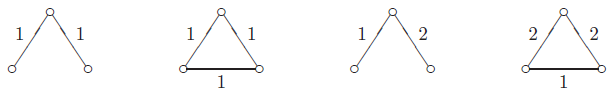
\includegraphics[scale = .65]{3vertconnected.PNG}
\caption{Unoriented 3-vertex connected subdiagrams}
\end{figure}
\end{lemma}

\end{frame}
\subsection{Possible mutations for 3-cycles in $\Gamma$}

\begin{frame}{Possible mutations for $i\--\ k\--\ j$}
\begin{corollary}
[Corollary 2.3, Barot-Marsh]
If in $\Gamma$ we have $i,j,k \in V(\Gamma), i \neq k \neq j$, and we have $i\--\ k\--\ j$, then the only possible mutations for this connected path between the three vertices are the following:
\begin{figure}[h]
\centering
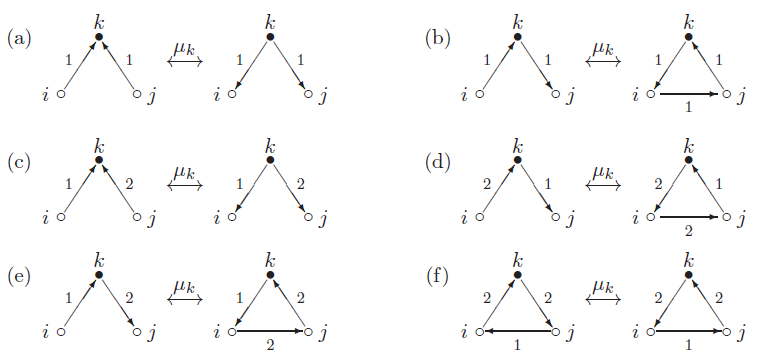
\includegraphics[scale = .40]{mutation3path.PNG}
\caption{Mutation of three connected vertices}
\end{figure}
\end{corollary}
\end{frame}

\begin{frame}{Sketch of Proof of the Main Theorem}
Now consider the diagram:
\begin{figure}
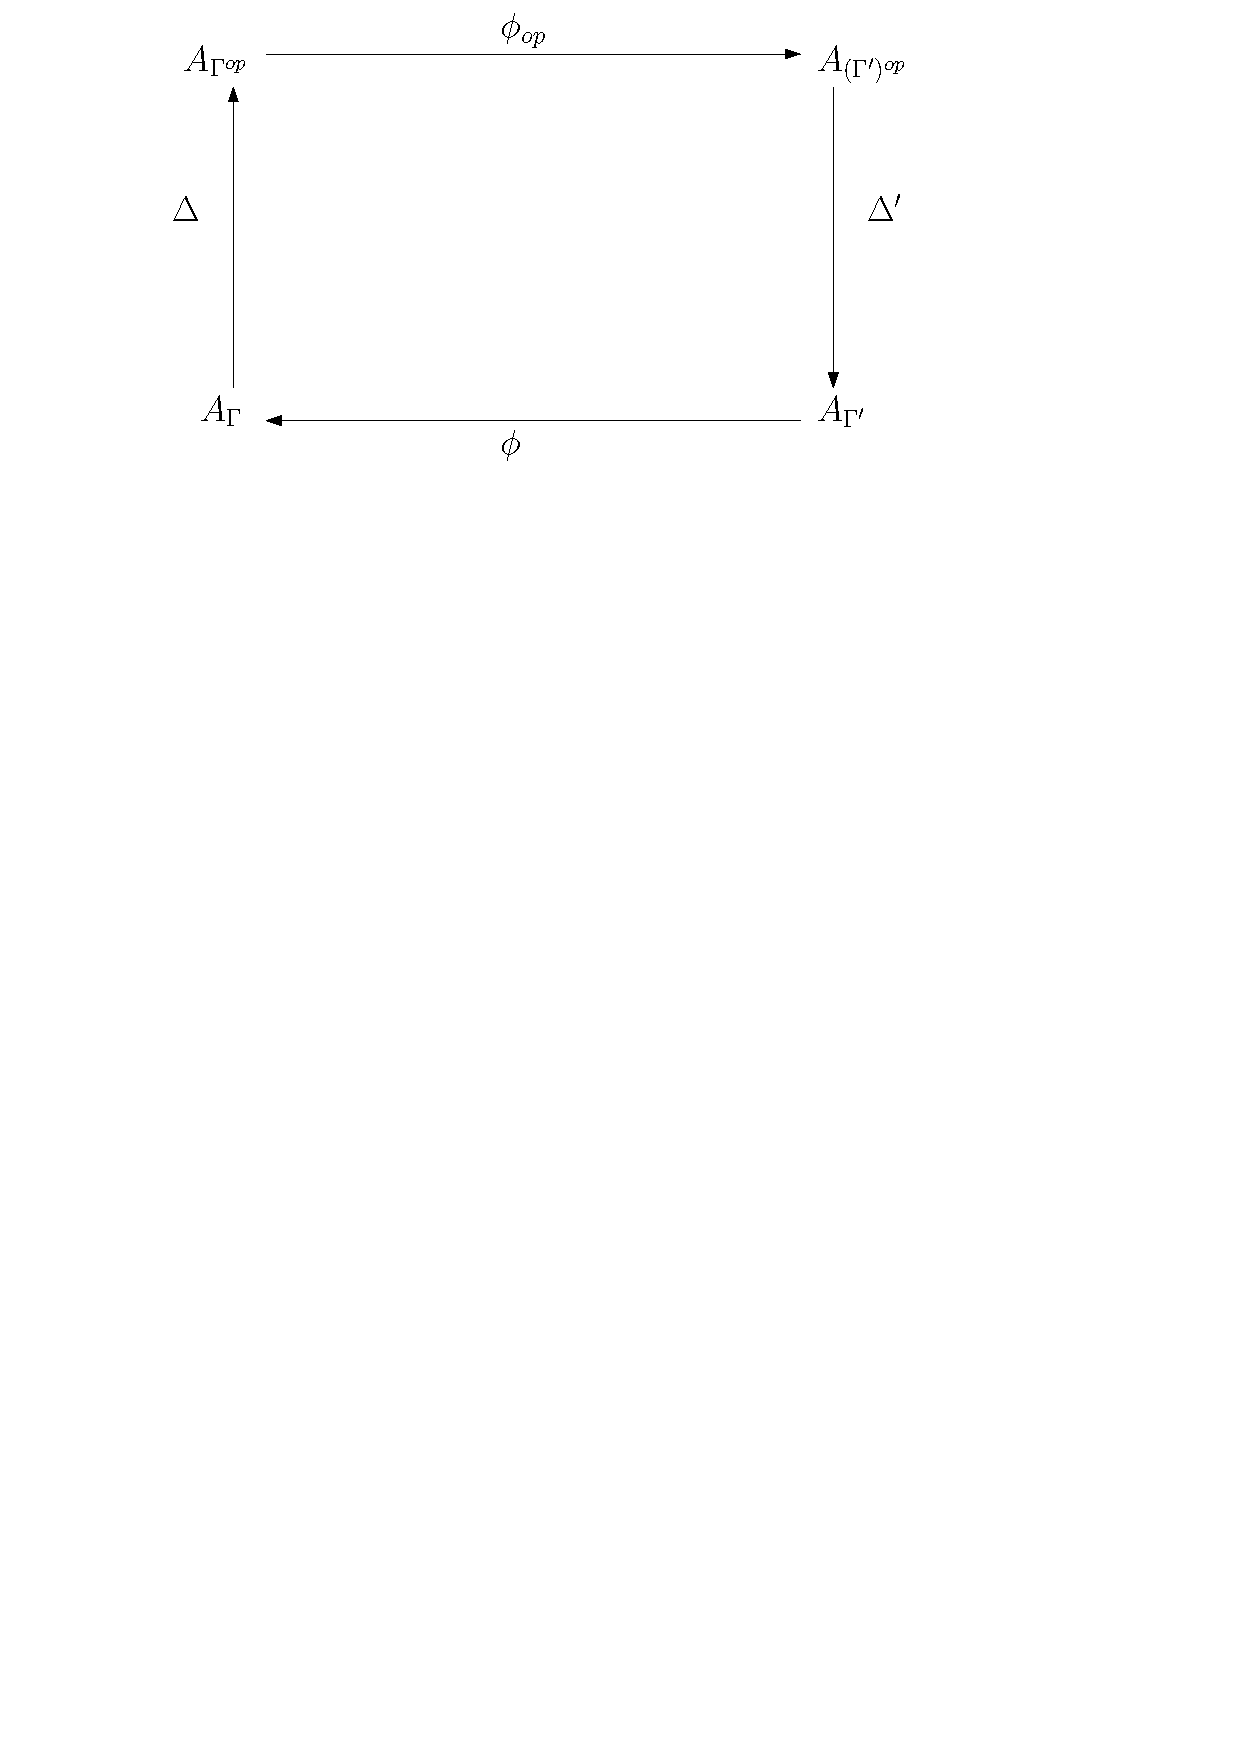
\includegraphics[scale = .50]{Comm-Diag.pdf}
\end{figure}
One can check that this diagram commutes, and so we find that the map $\phi$ is actually an isomorphism, which proves our theorem.
\end{frame}

\section{Affine Dynkin Diagrams}
\begin{frame}{Extending Result to Other Diagrams}
It is natural to ask whether a similar result holds for diagrams that are not of finite type. In particular, we will examine diagrams which are mutation equivalent to affine Dynkin diagrams.
\begin{figure}
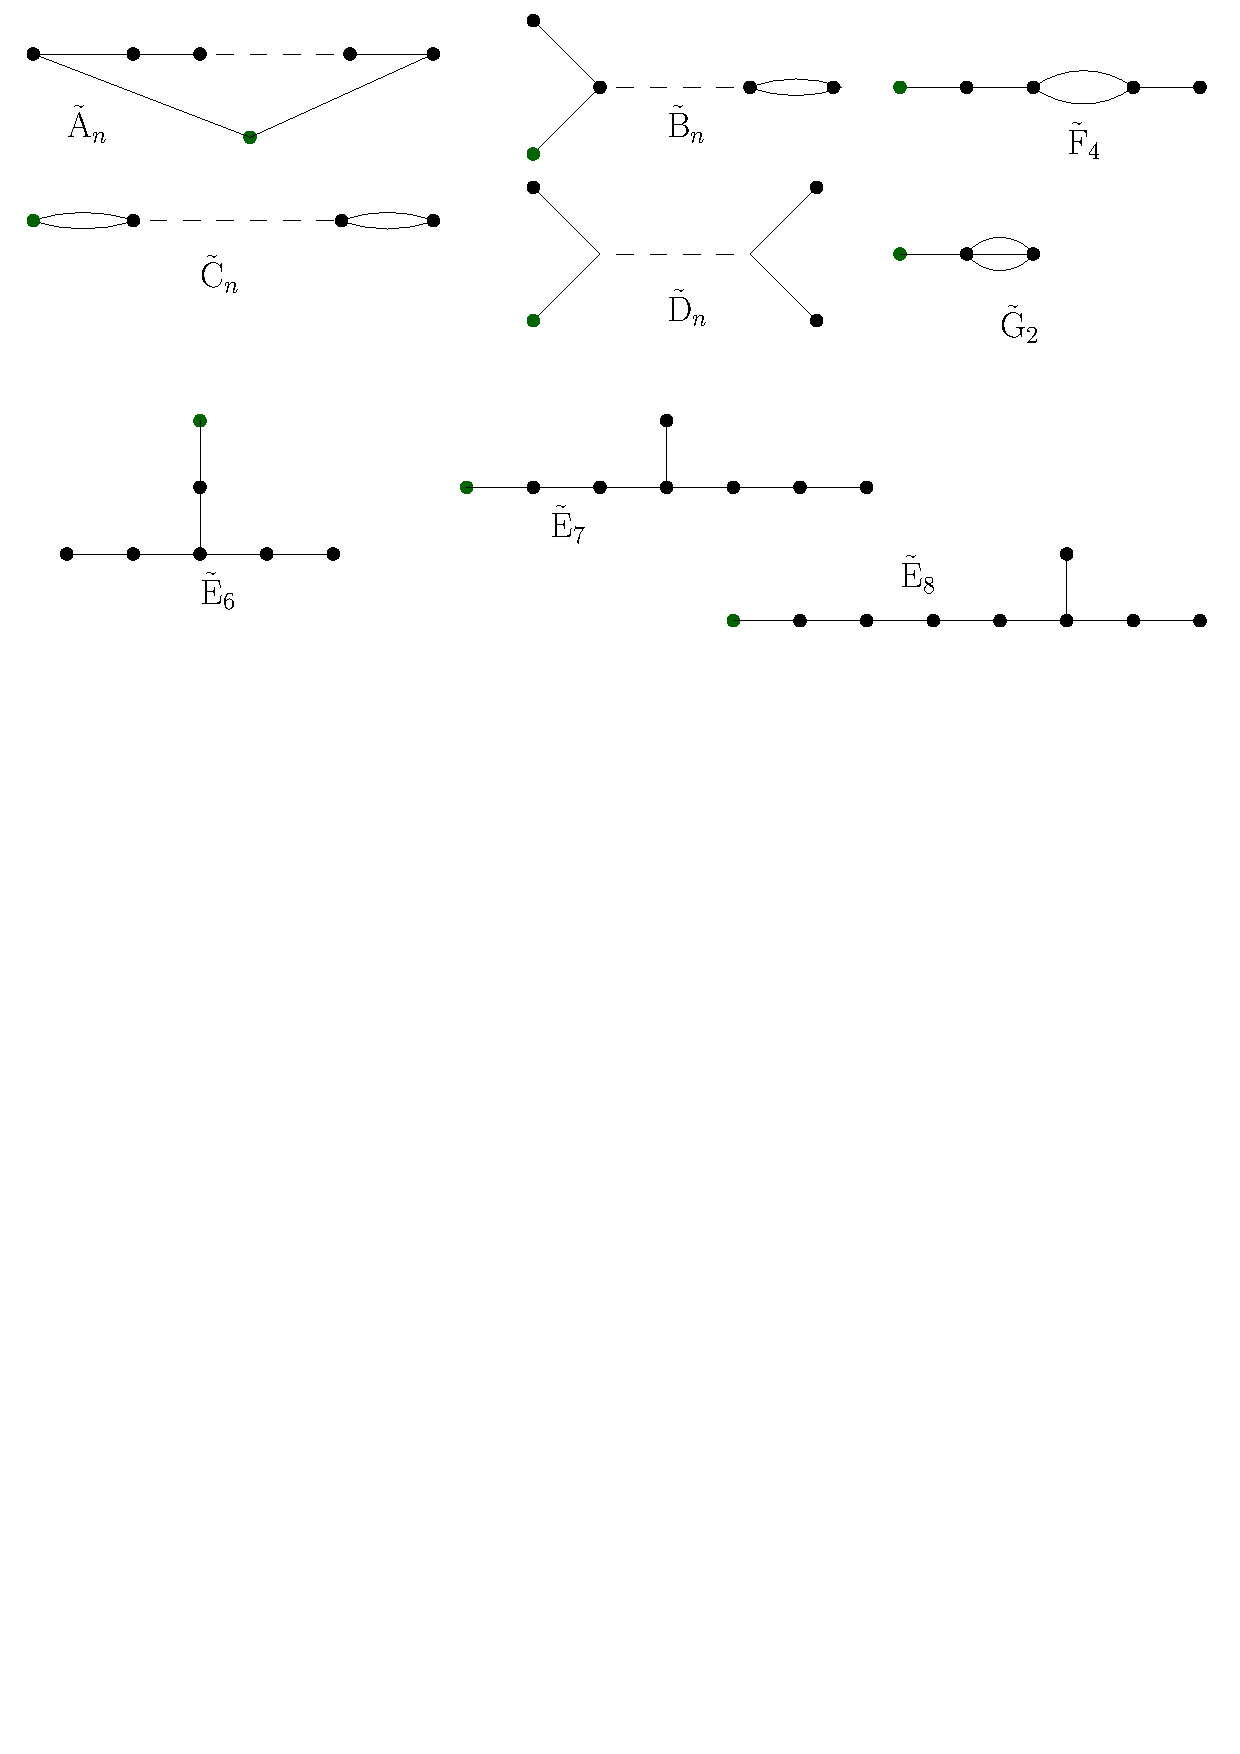
\includegraphics[scale = .50]{Affine-Diagrams.pdf}
\caption{Affine Dynkin Diagrams}
\end{figure}
\end{frame}

\begin{frame}{Extending the Barot-Marsh Presentation}
In a paper by Felickson and Tumarkin, the authors obtain a similar result for coxeter groups. For a diagram $\Gamma$ of affine type with n+1 nodes, they define a group W$_{\Gamma}$ generated by elements $s_{1}, \dots, s_{n+1}$ and subject to the following relations:

(R1) $s_{i}^{2} = e$ for $i \in \{1, \dots, n\}$.

(R2) $(s_{i}s_{j})^{m_{ij}} = e$ where 
$$m_{ij} = 
\begin{cases}
2 &\text{if there is no arrow between i and j in $\Gamma$} \\
3 &\text{if there is an arrow of weight 1 between i and j in $\Gamma$} \\
4 &\text{if there is an arrow of weight 2 between i and j in $\Gamma$} \\
6 &\text{if there is an arrow of weight 3 between i and j in $\Gamma$} \\
\infty &\text{otherwise}
\end{cases}$$
\end{frame}

\begin{frame}{Extending the Barot-Marsh Presentation}
(R3) For every chordless oriented cycle:
$$i_{0} \stackrel{w_{i_{0}}}{\longrightarrow} i_{1} \stackrel{w_{i_{1}}}{\longrightarrow} \dots \stackrel{w_{i_{d-2}}}{\longrightarrow} i_{d-1} \stackrel{w_{i_{d-1}}}{\longrightarrow} i_{0},$$
define for l $\in \{0, \dots, d-1\}$, 
$$t(l) = (\prod_{j=l}^{l+d-2}{\sqrt{w_{i_{j}}}} - \sqrt{w_{i_{l+d-1}}})^{2}.$$
Then take the relation $(s_{i_{l}}p(i_{l}, i_{l+1}))^{m(l)} = e$ where
$$m(l) =
\begin{cases}
2 &\text{if $t(l)=0$} \\
3 &\text{if $t(l)=1$} \\
4 &\text{if $t(l)=2$} \\
6 &\text{if $t(l)=3$}
\end{cases}$$
\end{frame}

\begin{frame}{Extending the Barot-Marsh Presentation}
(R4) To a subdiagram of the form
\begin{figure}
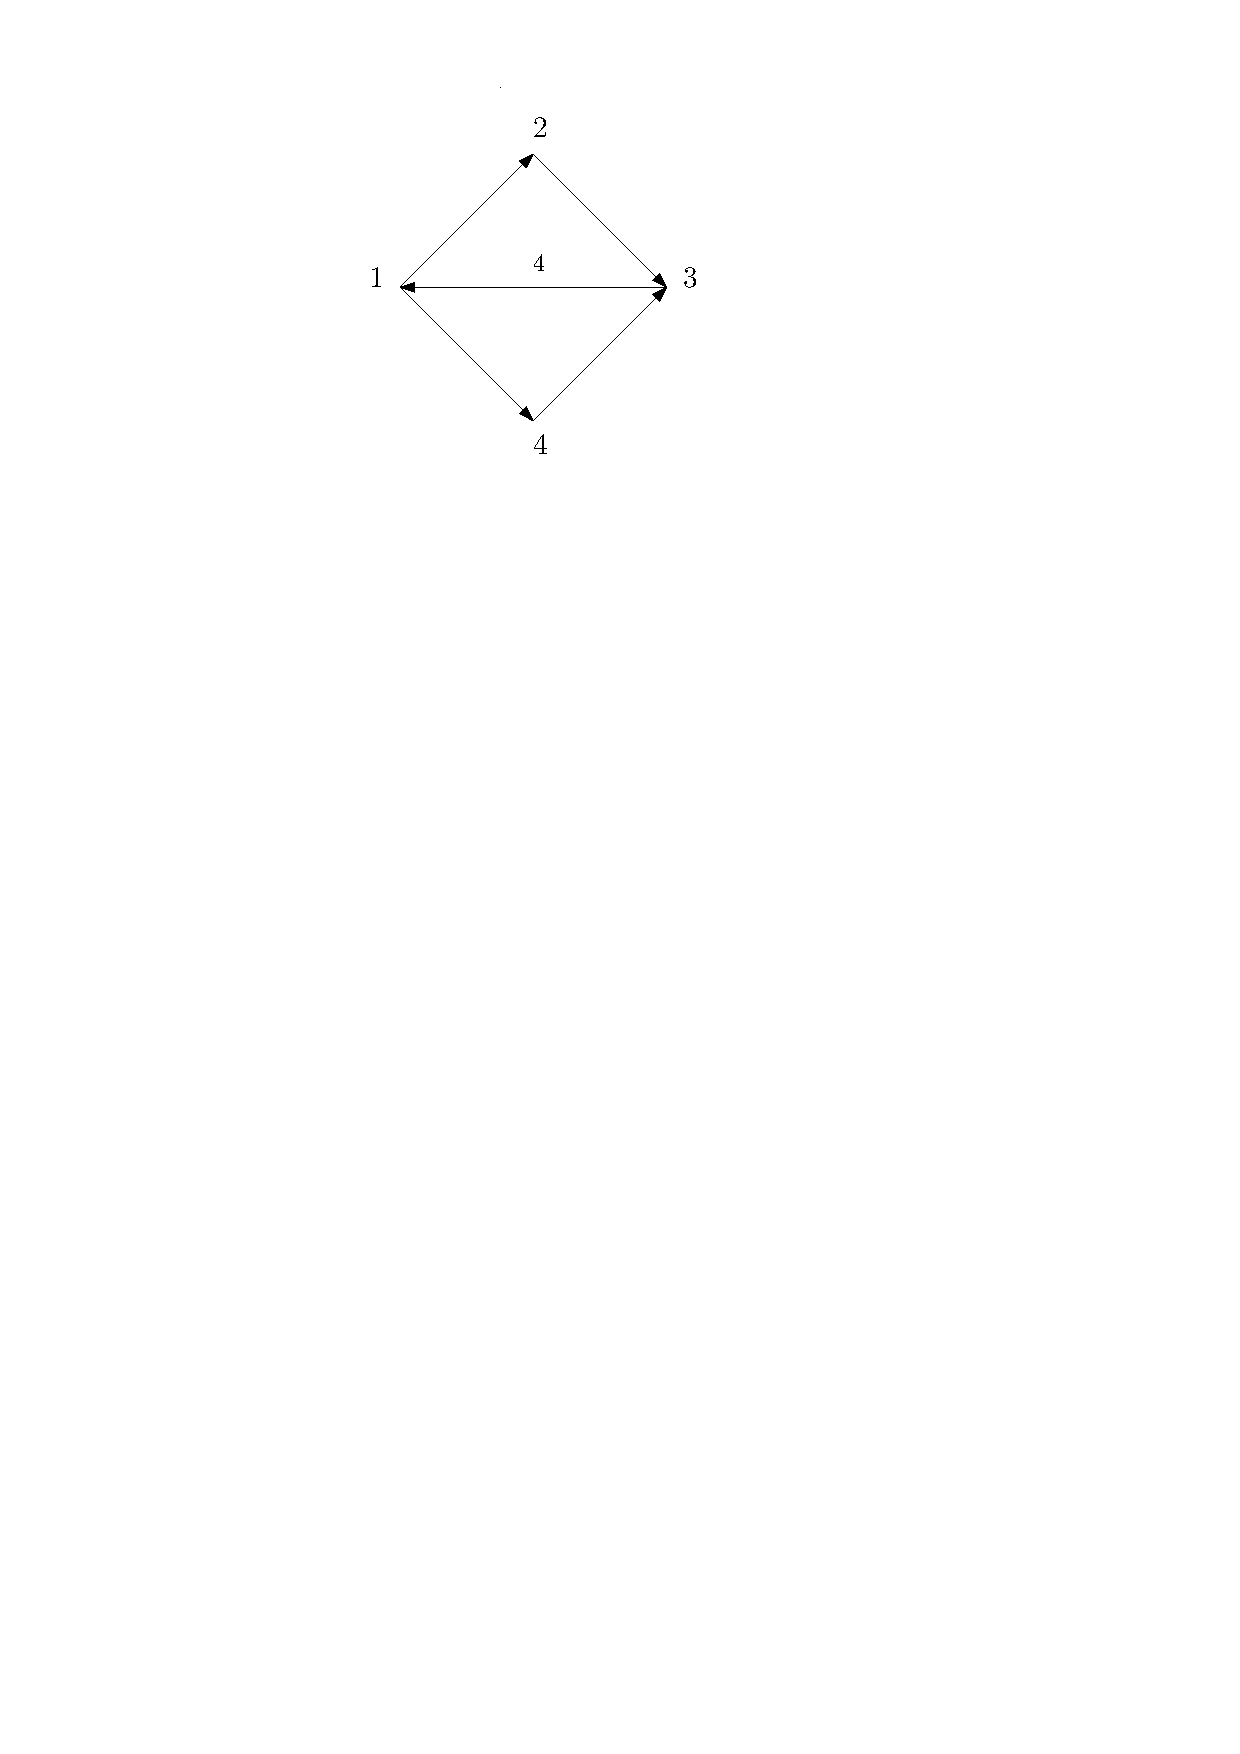
\includegraphics[scale = .50]{Diagram1.pdf}
\end{figure}
we add the relation $(s_{1}s_{2}s_{3}s_{4}s_{3}s_{2})^{2} = e$.
\end{frame}

\begin{frame}{Extending the Barot-Marsh Presentation}
To a subdiagram of the form 
\begin{figure}
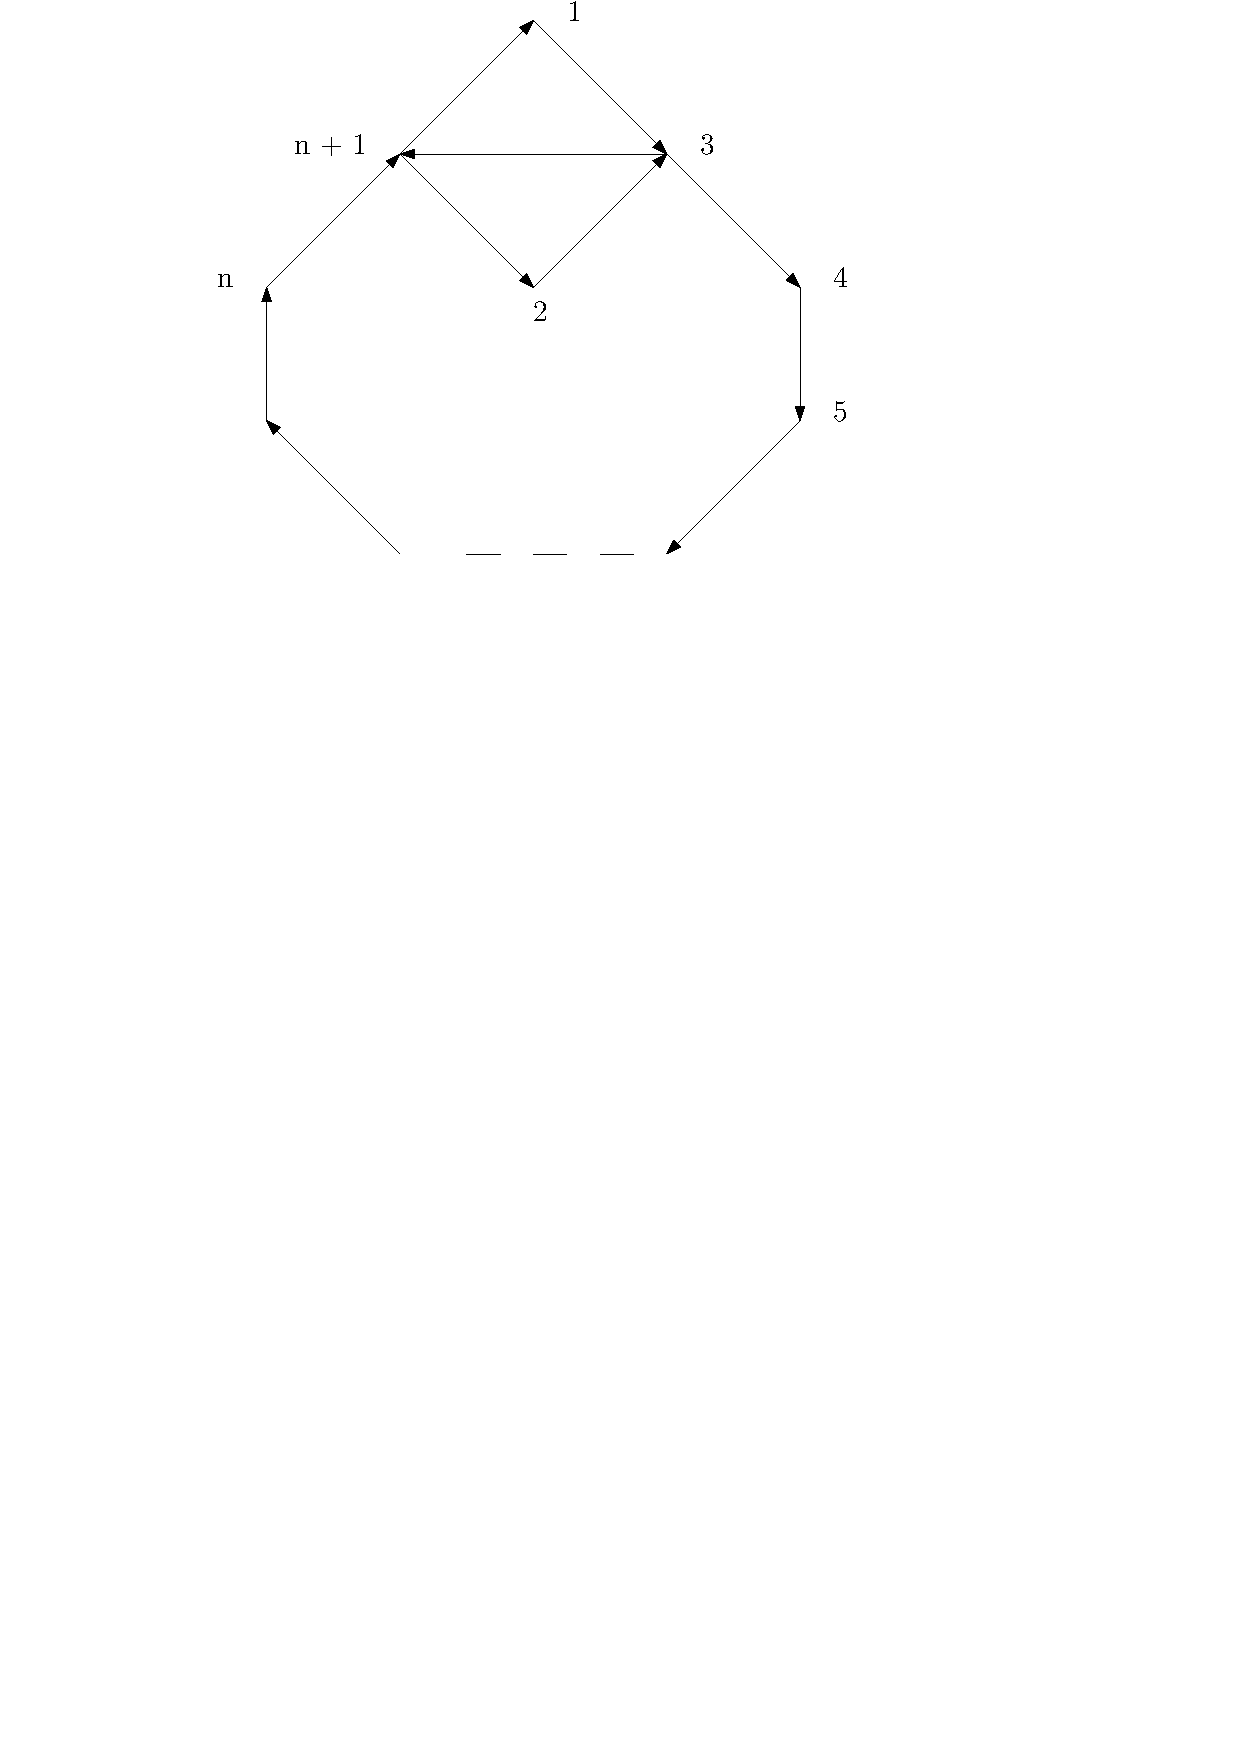
\includegraphics[scale = .50]{Diagram2.pdf}
\end{figure}
we add the relation $(s_{1}s_{2}s_{3}s_{2}s_{1}s_{4}s_{5} \dots s_{n}s_{n+1}s_{n} \dots s_{5}s_{4})^{2} = e$
\end{frame}

\begin{frame}{Extending the Barot-Marsh Presentation}
To a subdiagram of the form
\begin{figure}
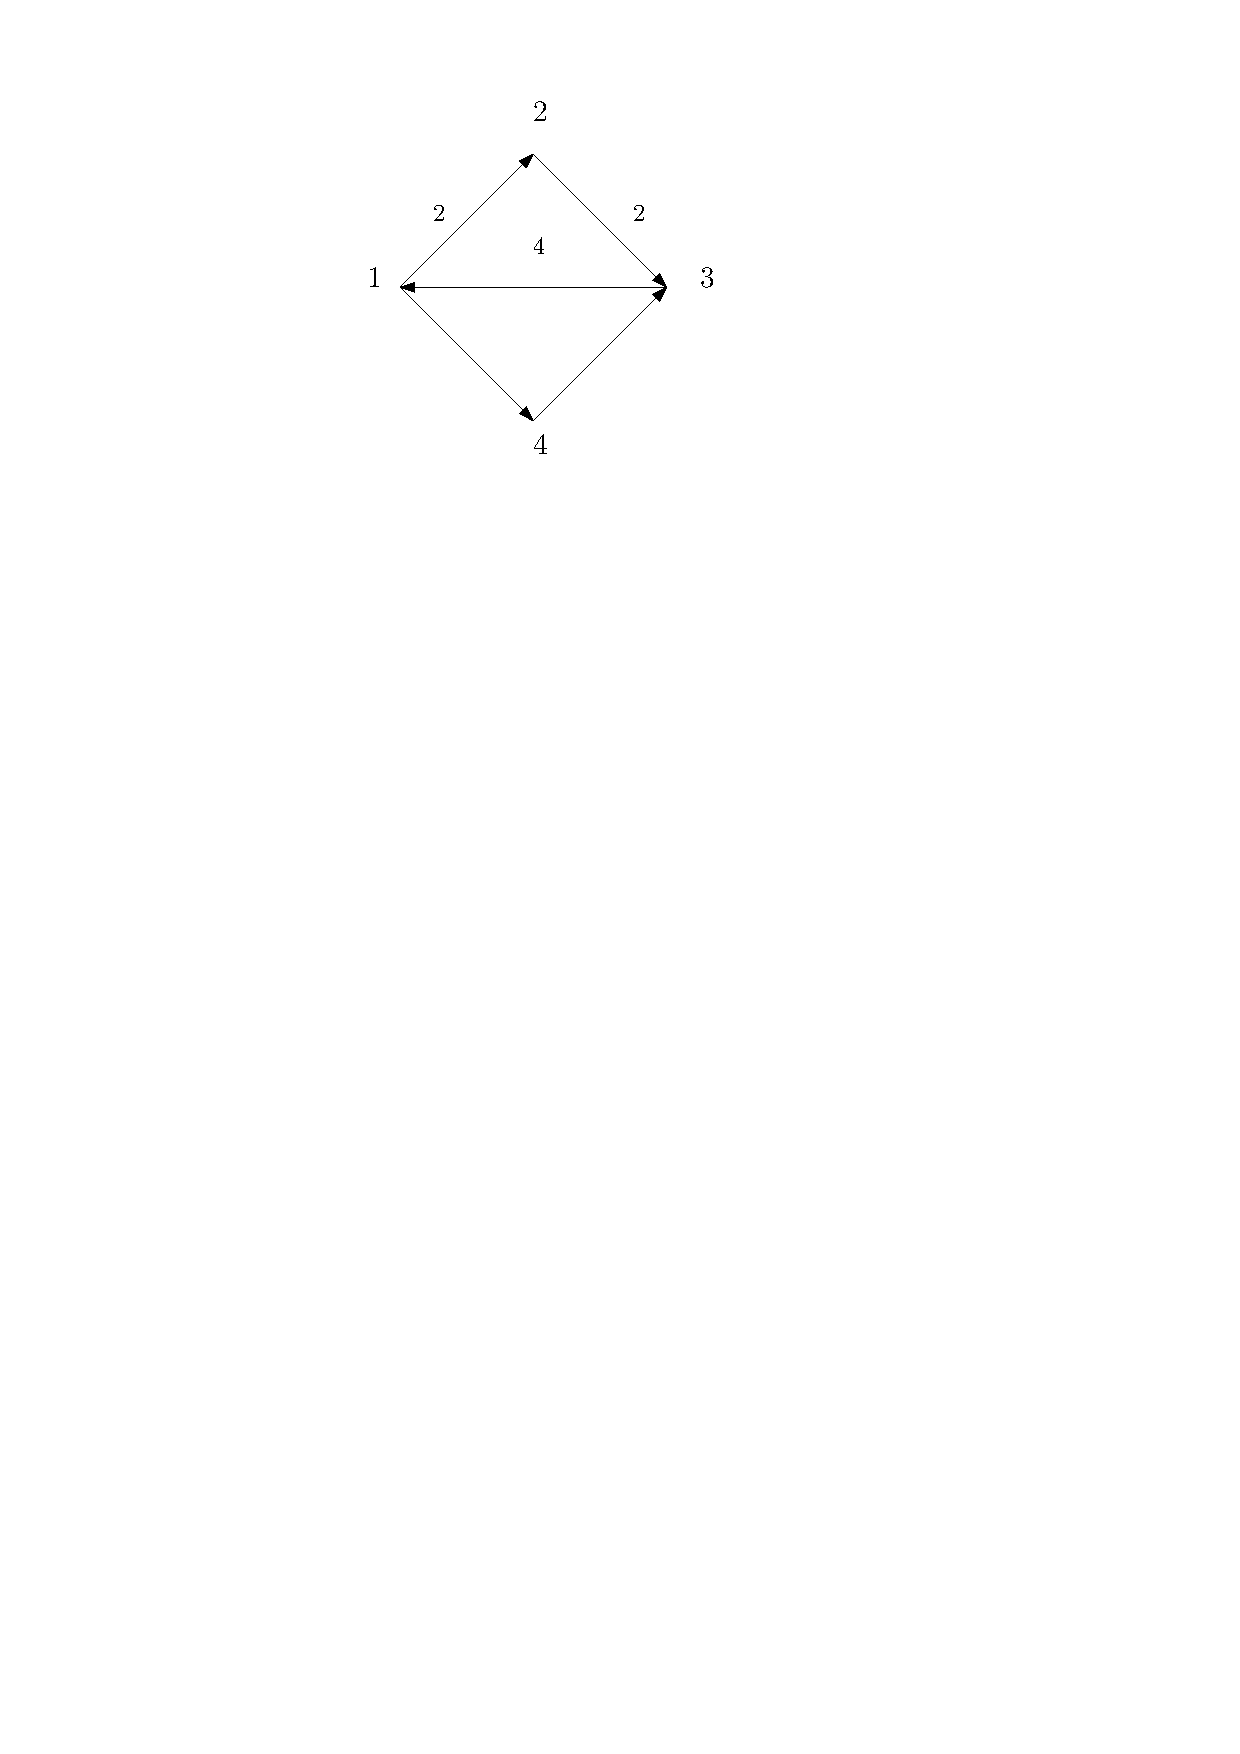
\includegraphics[scale = .50]{Diagram3.pdf}
\end{figure}
we add the relations $(s_{2}s_{3}s_{4}s_{1}s_{4}s_{3})^{2} = e$ and $(s_{2}s_{1}s_{4}s_{3}s_{4}s_{1})^{2} = e$.
\end{frame}

\begin{frame}{Extending the Barot-Marsh Presentation}
To a subdiagram of the form
\begin{figure}
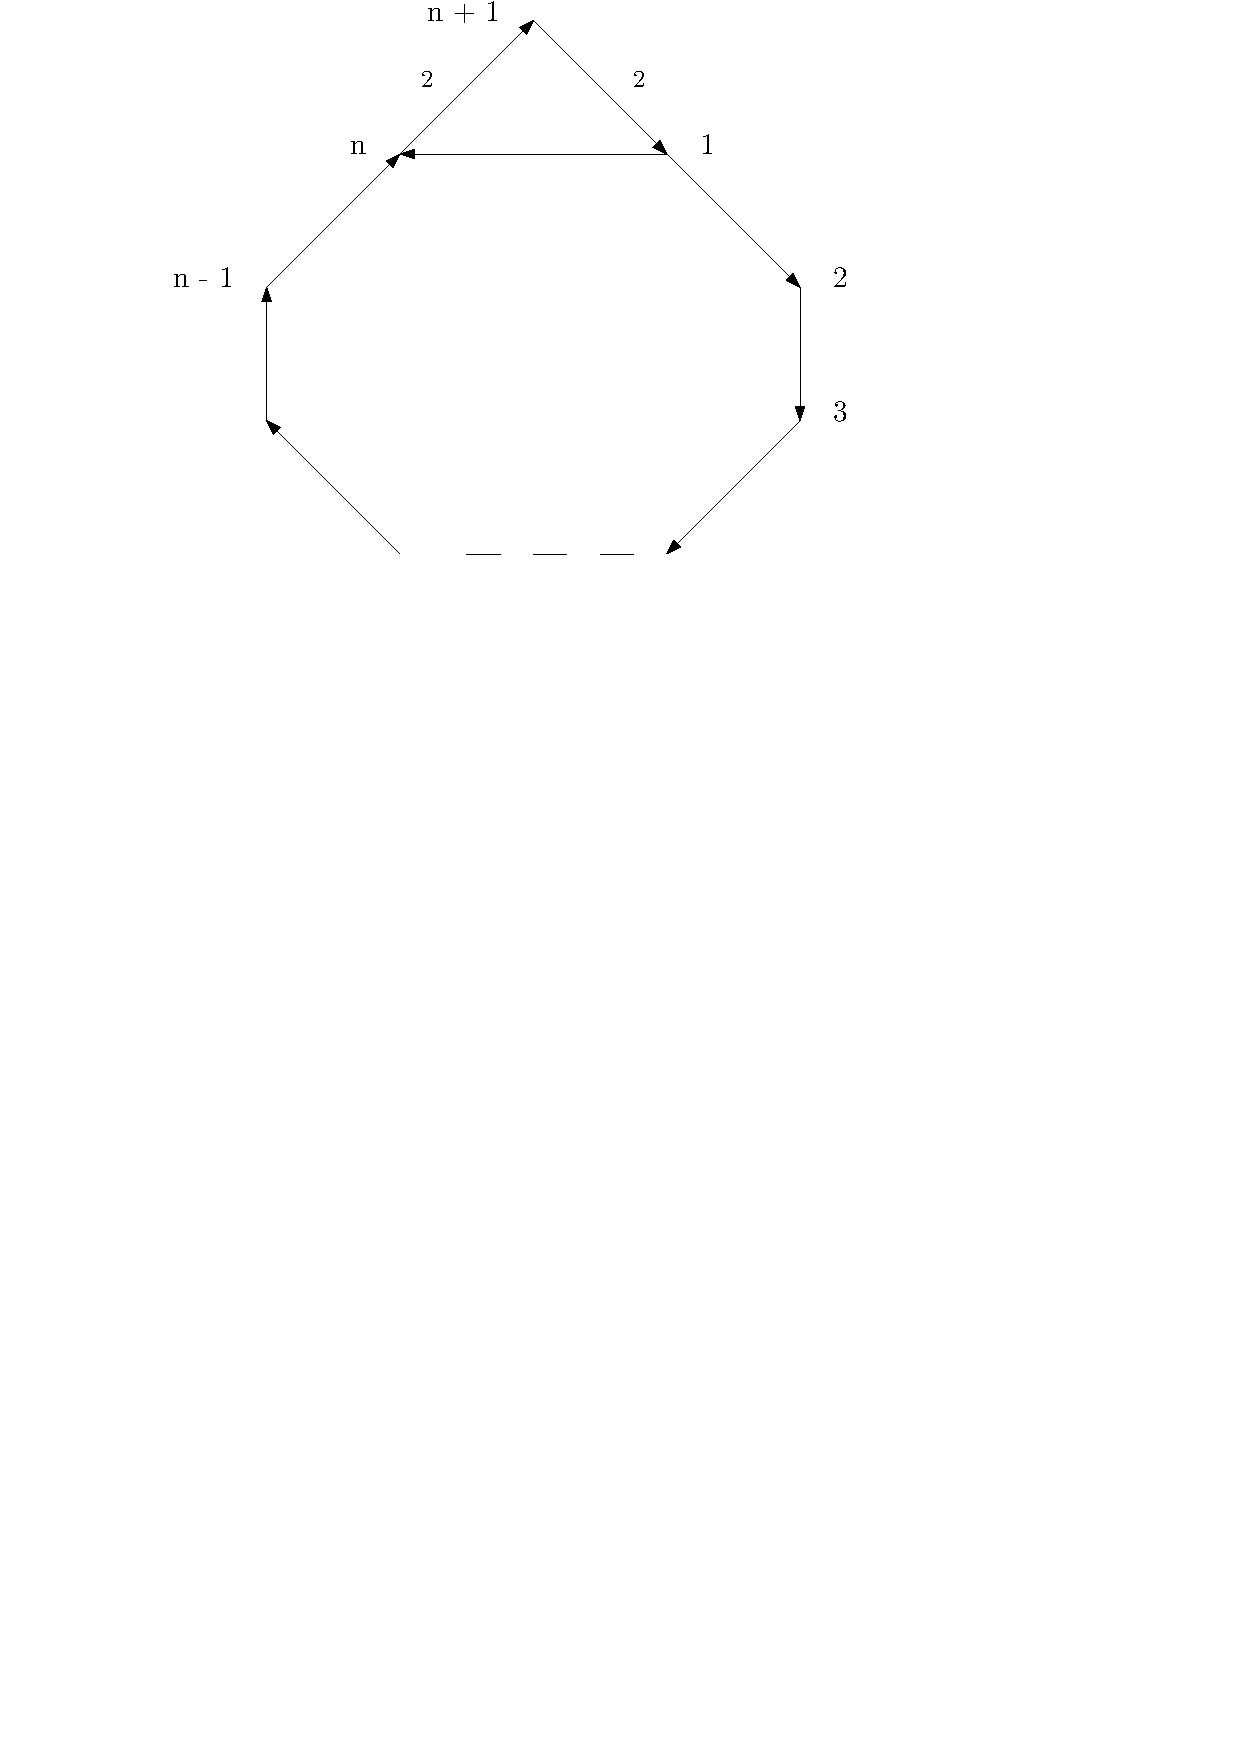
\includegraphics[scale = .50]{Diagram4.pdf}
\end{figure}
we add the relation $(s_{n+1}s_{1}s_{n+1}s_{2}s_{3} \dots s_{n-1}s_{n}s_{n-1} \dots s_{3}s_{2})^{2} = e$.
\end{frame}

\begin{frame}{Extending the Barot-Marsh Presentation}
To a subdiagram of the form
\begin{figure}
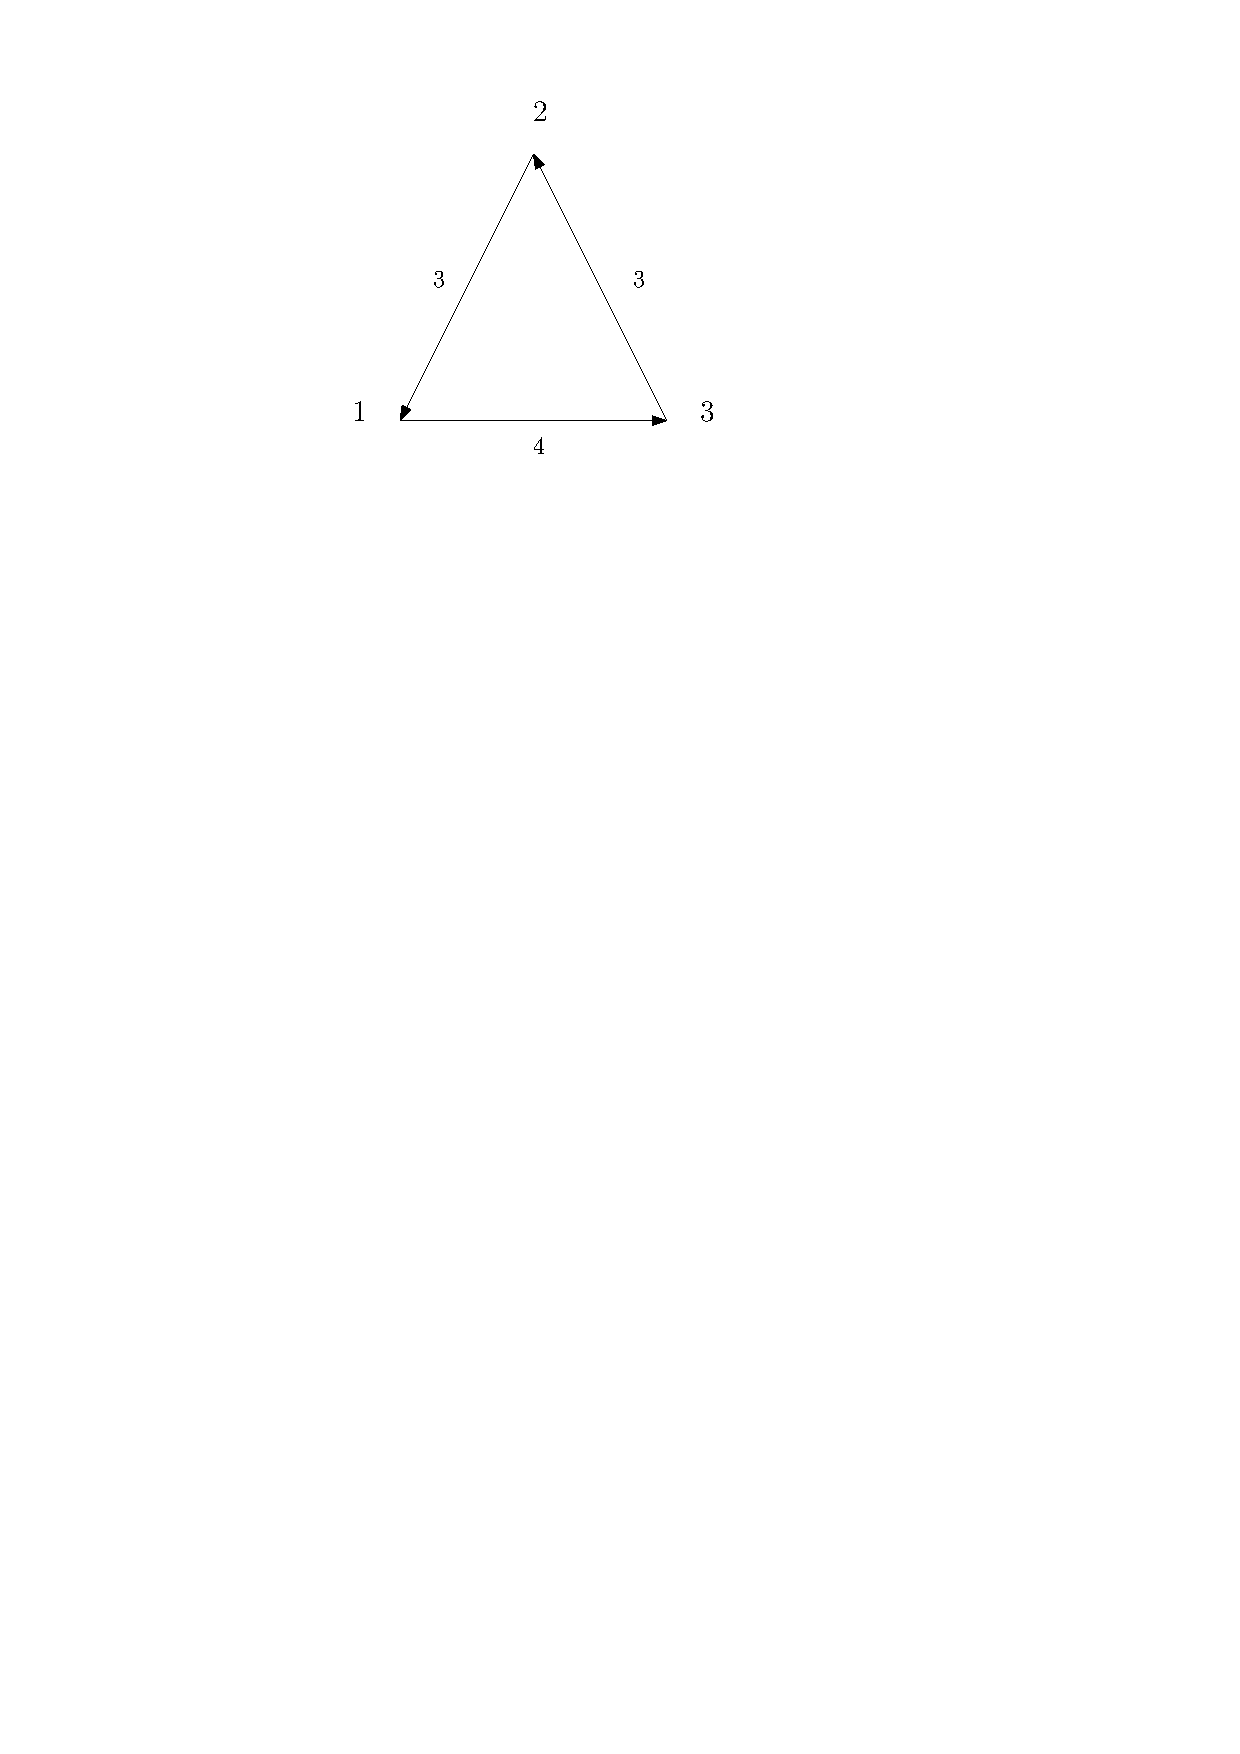
\includegraphics[scale = .50]{Diagram5.pdf}
\end{figure}
we add the relations $(s_{2}s_{1}s_{2}s_{1}s_{2}s_{3})^{2} = e$ and $(s_{2}s_{3}s_{2}s_{3}s_{2}s_{1})^{2} = e$
\end{frame}

\begin{frame}
\begin{theorem}[Felickson-Tumarkin]
The group $W_{\Gamma}$ is invariant up to isomorphism under diagram mutation.
\end{theorem}
\end{frame}

\begin{frame}{Purpose of (R4) Relations}
In their paper, Felickson and Tumarkin show that all of the (R4) relations are necessary for this theorem to be true. For example, consider the mutation of 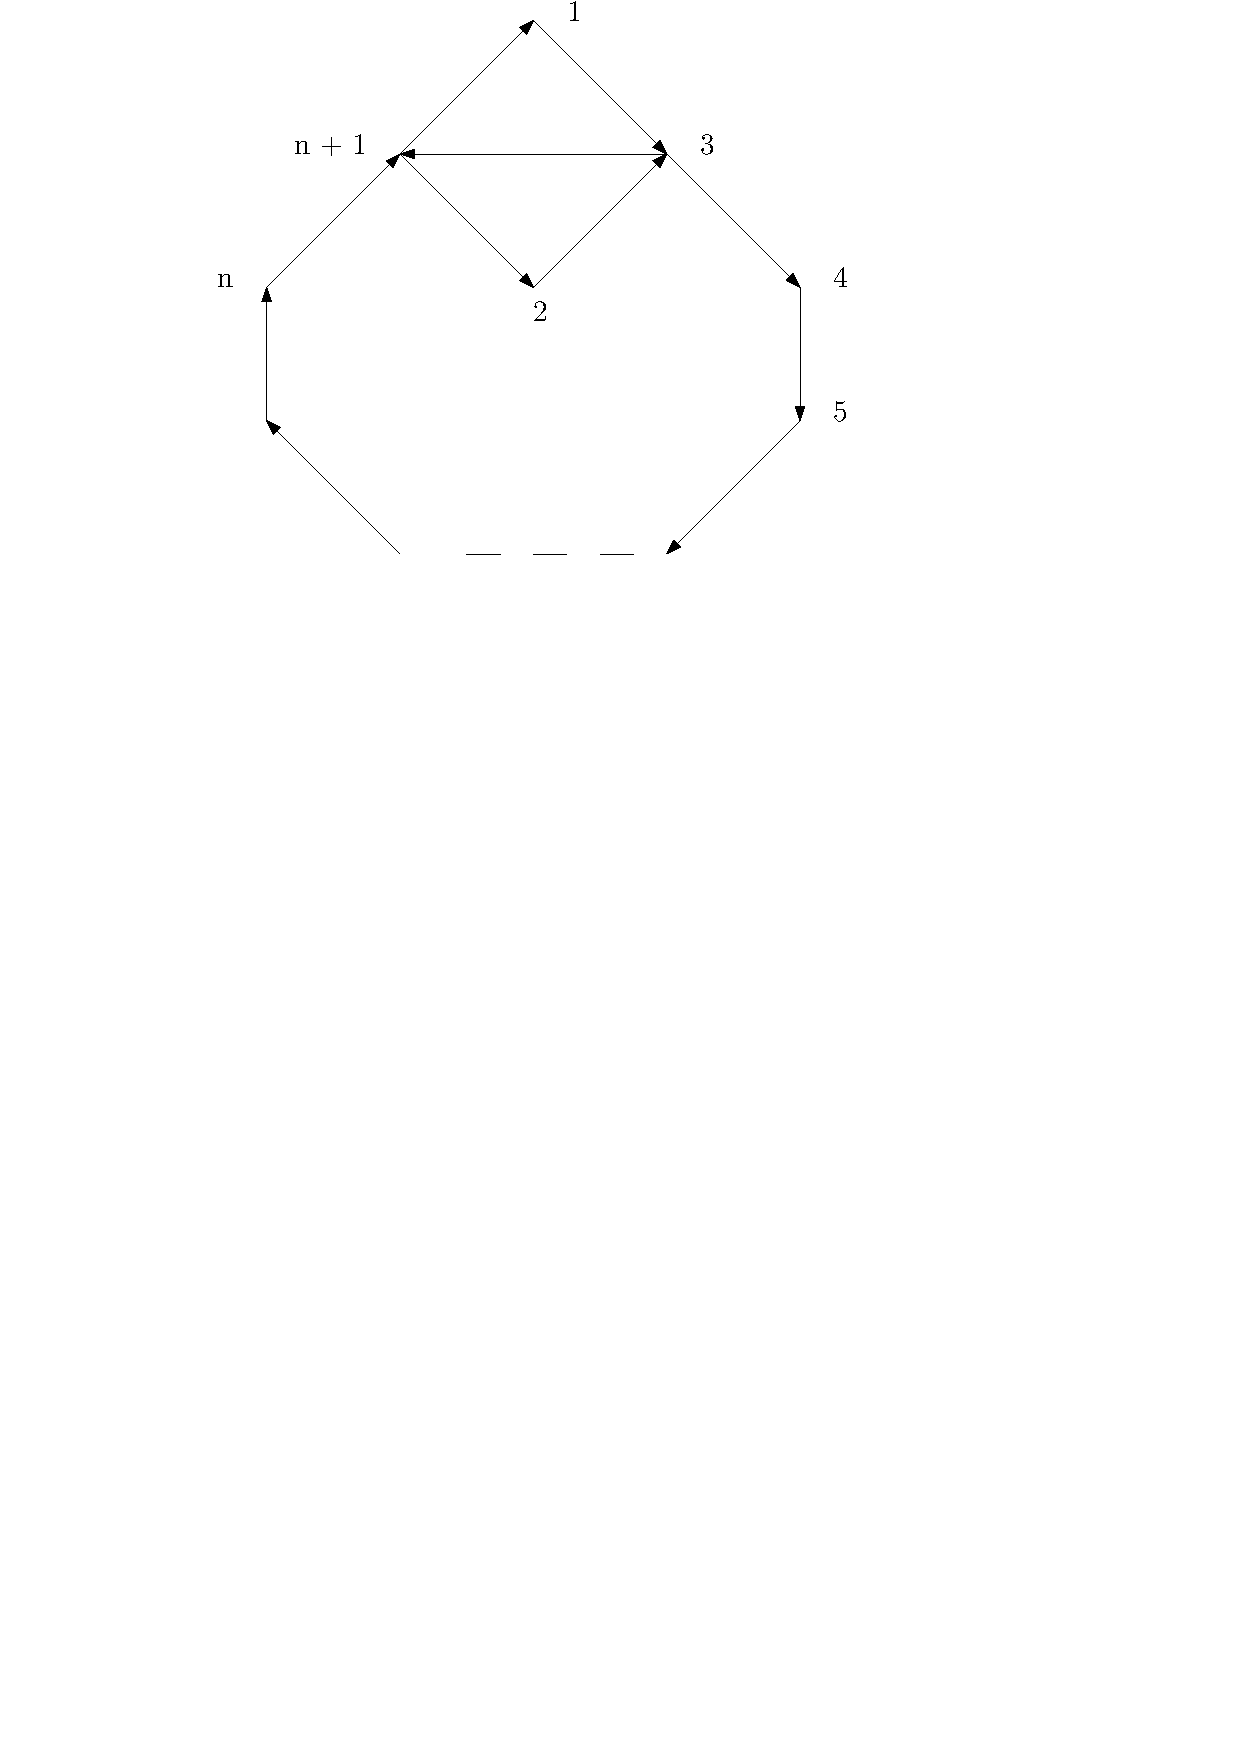
\includegraphics[scale = .30]{Diagram2.pdf} at the vertex 1, which is the diagram
\begin{figure}
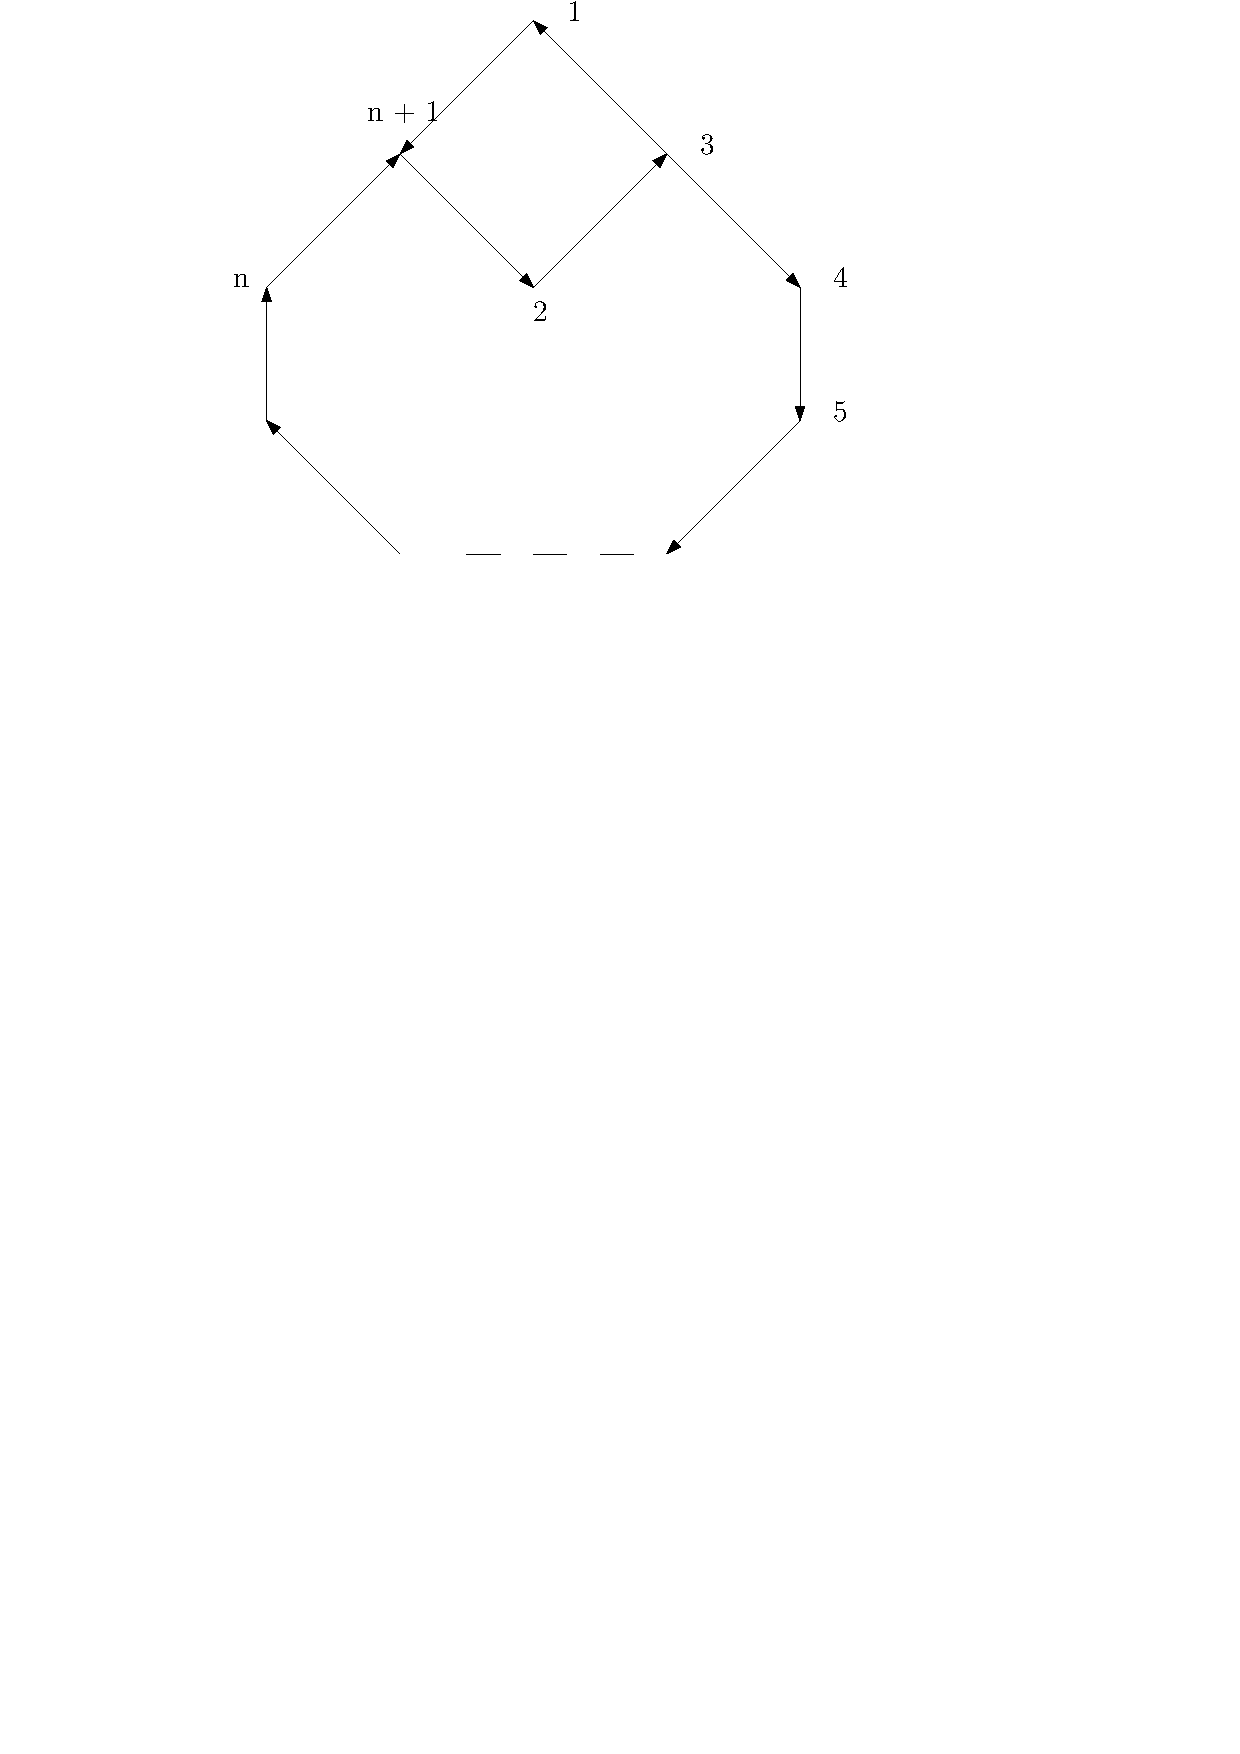
\includegraphics[scale = .30]{Diagram6.pdf}
\end{figure}
\end{frame}

\begin{frame}{Extending our Artin Group Presentations}
Let $\Gamma$ be a diagram of affine type on n+1 nodes. Then we define $A_{\Gamma}$ to be the group generated by $s_{1}, \dots, s_{n+1}$ satisfying the relations

(T2) $\langle s_{i}, s_{j} \rangle^{m_{ij}} = \langle s_{j}, s_{i} \rangle^{m_{ij}}$ where
$$m_{ij} = 
\begin{cases}
2 &\text{if there is no arrow between i and j in $\Gamma$} \\
3 &\text{if there is an arrow of weight 1 between i and j in $\Gamma$} \\
4 &\text{if there is an arrow of weight 2 between i and j in $\Gamma$} \\
6 &\text{if there is an arrow of weight 3 between i and j in $\Gamma$} \\
\infty &\text{otherwise}
\end{cases}$$
\end{frame}

\begin{frame}{Extending our Artin Group Presentations}
(T3)  For every chordless oriented cycle:
$$i_{0} \stackrel{w_{i_{0}}}{\longrightarrow} i_{1} \stackrel{w_{i_{1}}}{\longrightarrow} \dots \stackrel{w_{i_{d-2}}}{\longrightarrow} i_{d-1} \stackrel{w_{i_{d-1}}}{\longrightarrow} i_{0},$$
define for l $\in \{0, \dots, d-1\}$, 
$$t(l) = (\prod_{j=l}^{l+d-2}{\sqrt{w_{i_{j}}}} - \sqrt{w_{i_{l+d-1}}})^{2}.$$
Then take the relation $\langle s_{i_{l}}p(i_{l}, i_{l+1}) \rangle^{m(l)} = \langle p(i_{l}, i_{l+1})s_{i_{l}} \rangle^{m(l)}$ where
$$m(l) =
\begin{cases}
2 &\text{if $t(l)=0$} \\
3 &\text{if $t(l)=1$} \\
4 &\text{if $t(l)=2$} \\
6 &\text{if $t(l)=3$}
\end{cases}$$
\end{frame}

\begin{frame}{Extending our Artin Group Presentations}
(T4) To a subdiagram of the form
\begin{figure}
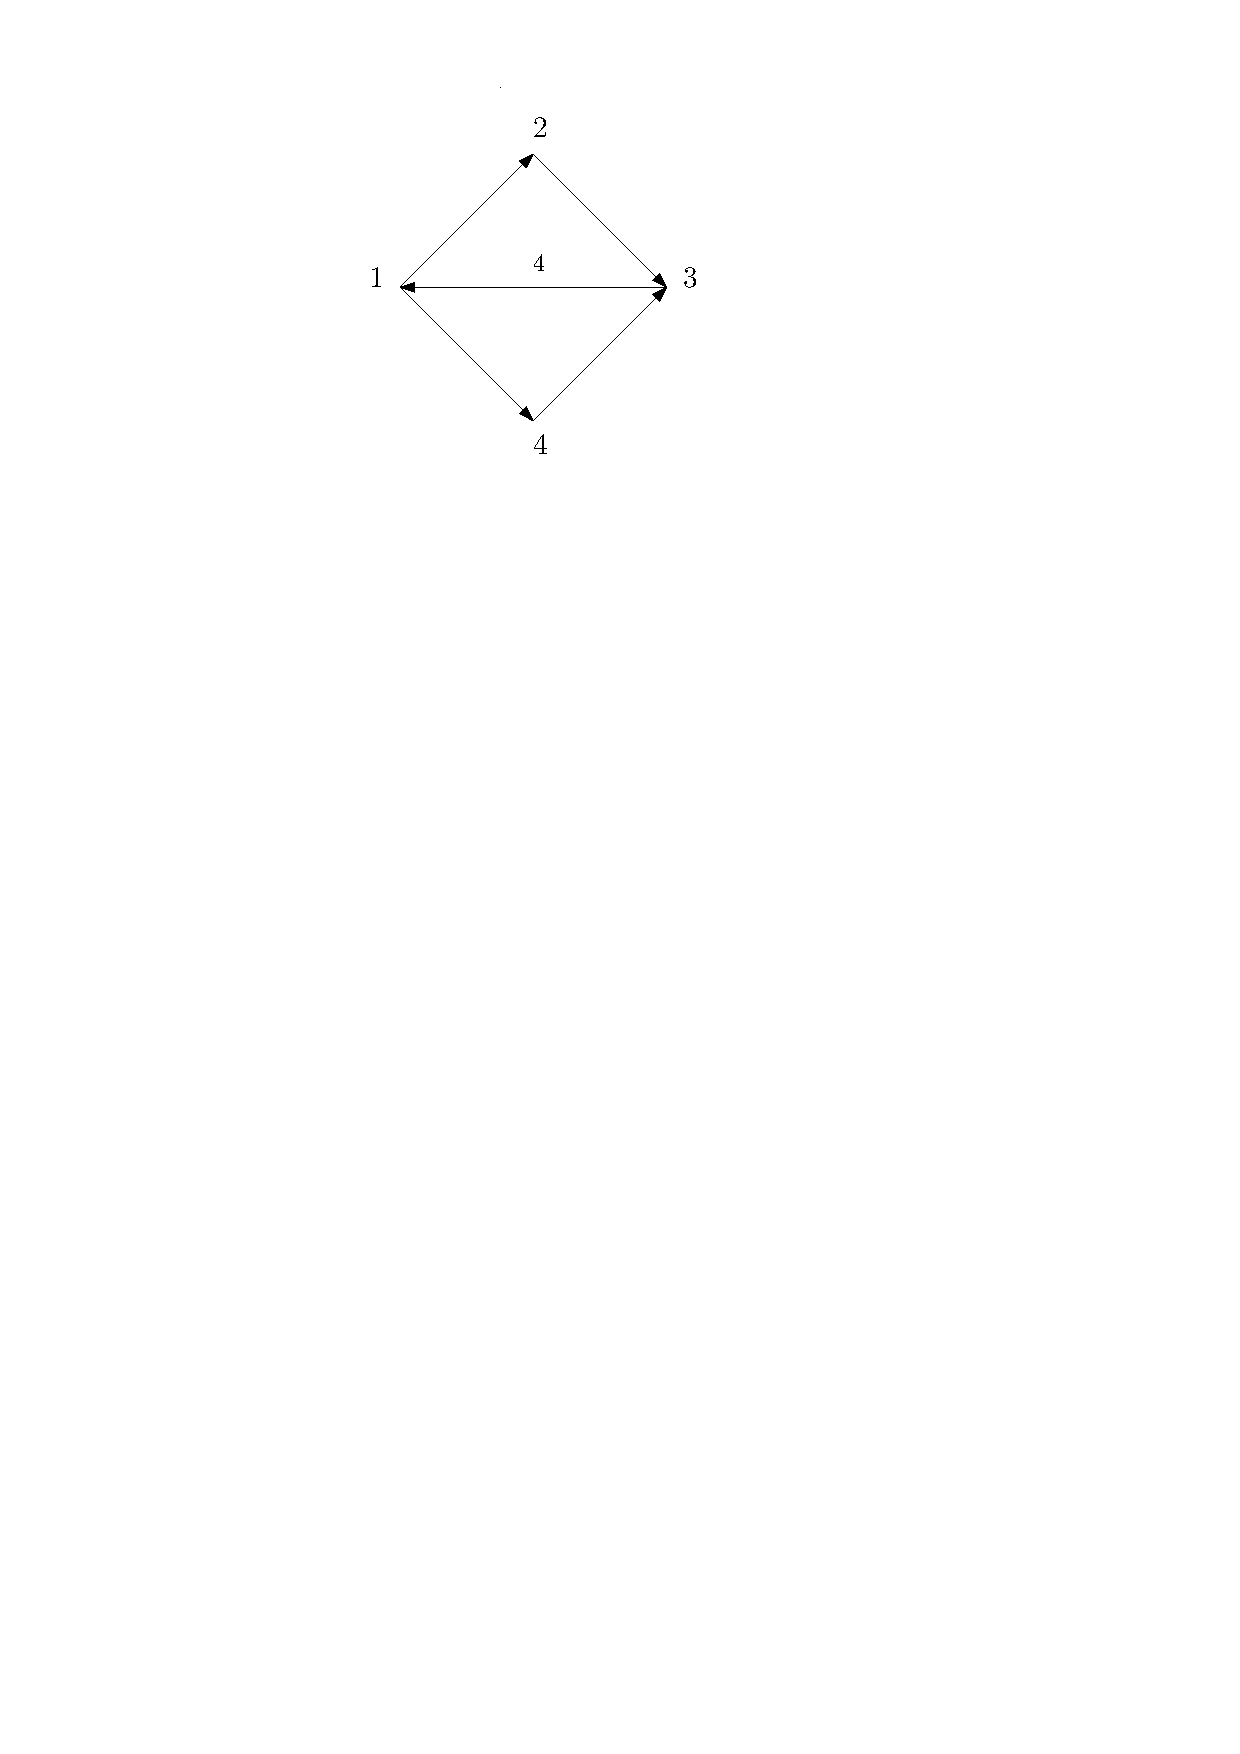
\includegraphics[scale = .50]{Diagram1.pdf}
\end{figure}
we add the relation $(s_{2}s_{1}s_{2}^{-1})s_{4}^{-1}s_{3}s_{4} = s_{4}^{-1}s_{3}s_{4}(s_{2}s_{1}s_{2}^{-1}).$
\end{frame}

\begin{frame}{Extending our Artin Group Presentations}
To a subdiagram of the form
\begin{figure}
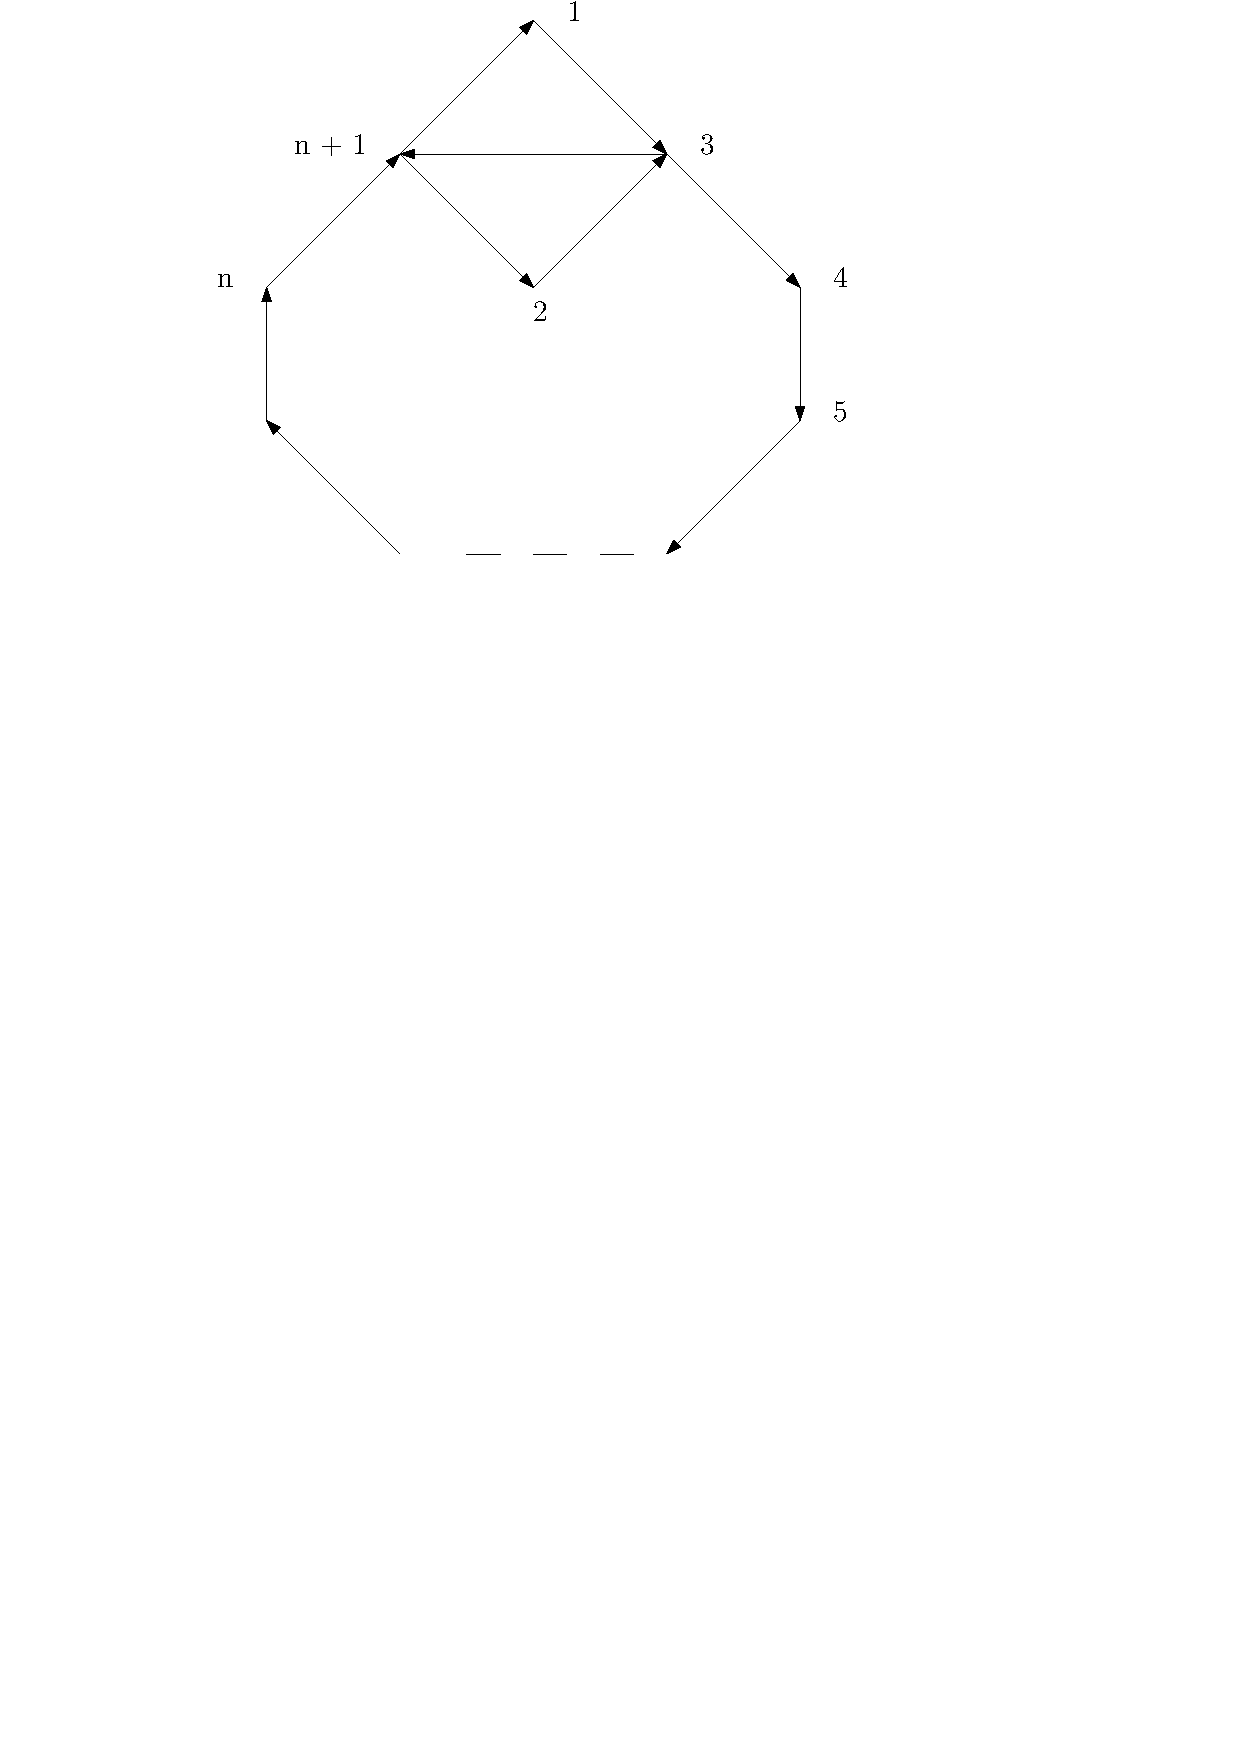
\includegraphics[scale = .50]{Diagram2.pdf}
\end{figure}
we add the relation
$s_{2}(s_{3}^{-1}s_{4}^{-1}\dots s_{n}^{-1}(s_{1}s_{n+1}s_{1}^{-1})s_{n} \dots s_{4}s_{3})$
\newline $= (s_{3}^{-1}s_{4}^{-1}\dots s_{n}^{-1}(s_{1}s_{n+1}s_{1}^{-1})s_{n} \dots s_{4}s_{3})s_{2}$
\end{frame}

\begin{frame}{Extending our Artin Group Presentations}
To a subdiagram of the form
\begin{figure}
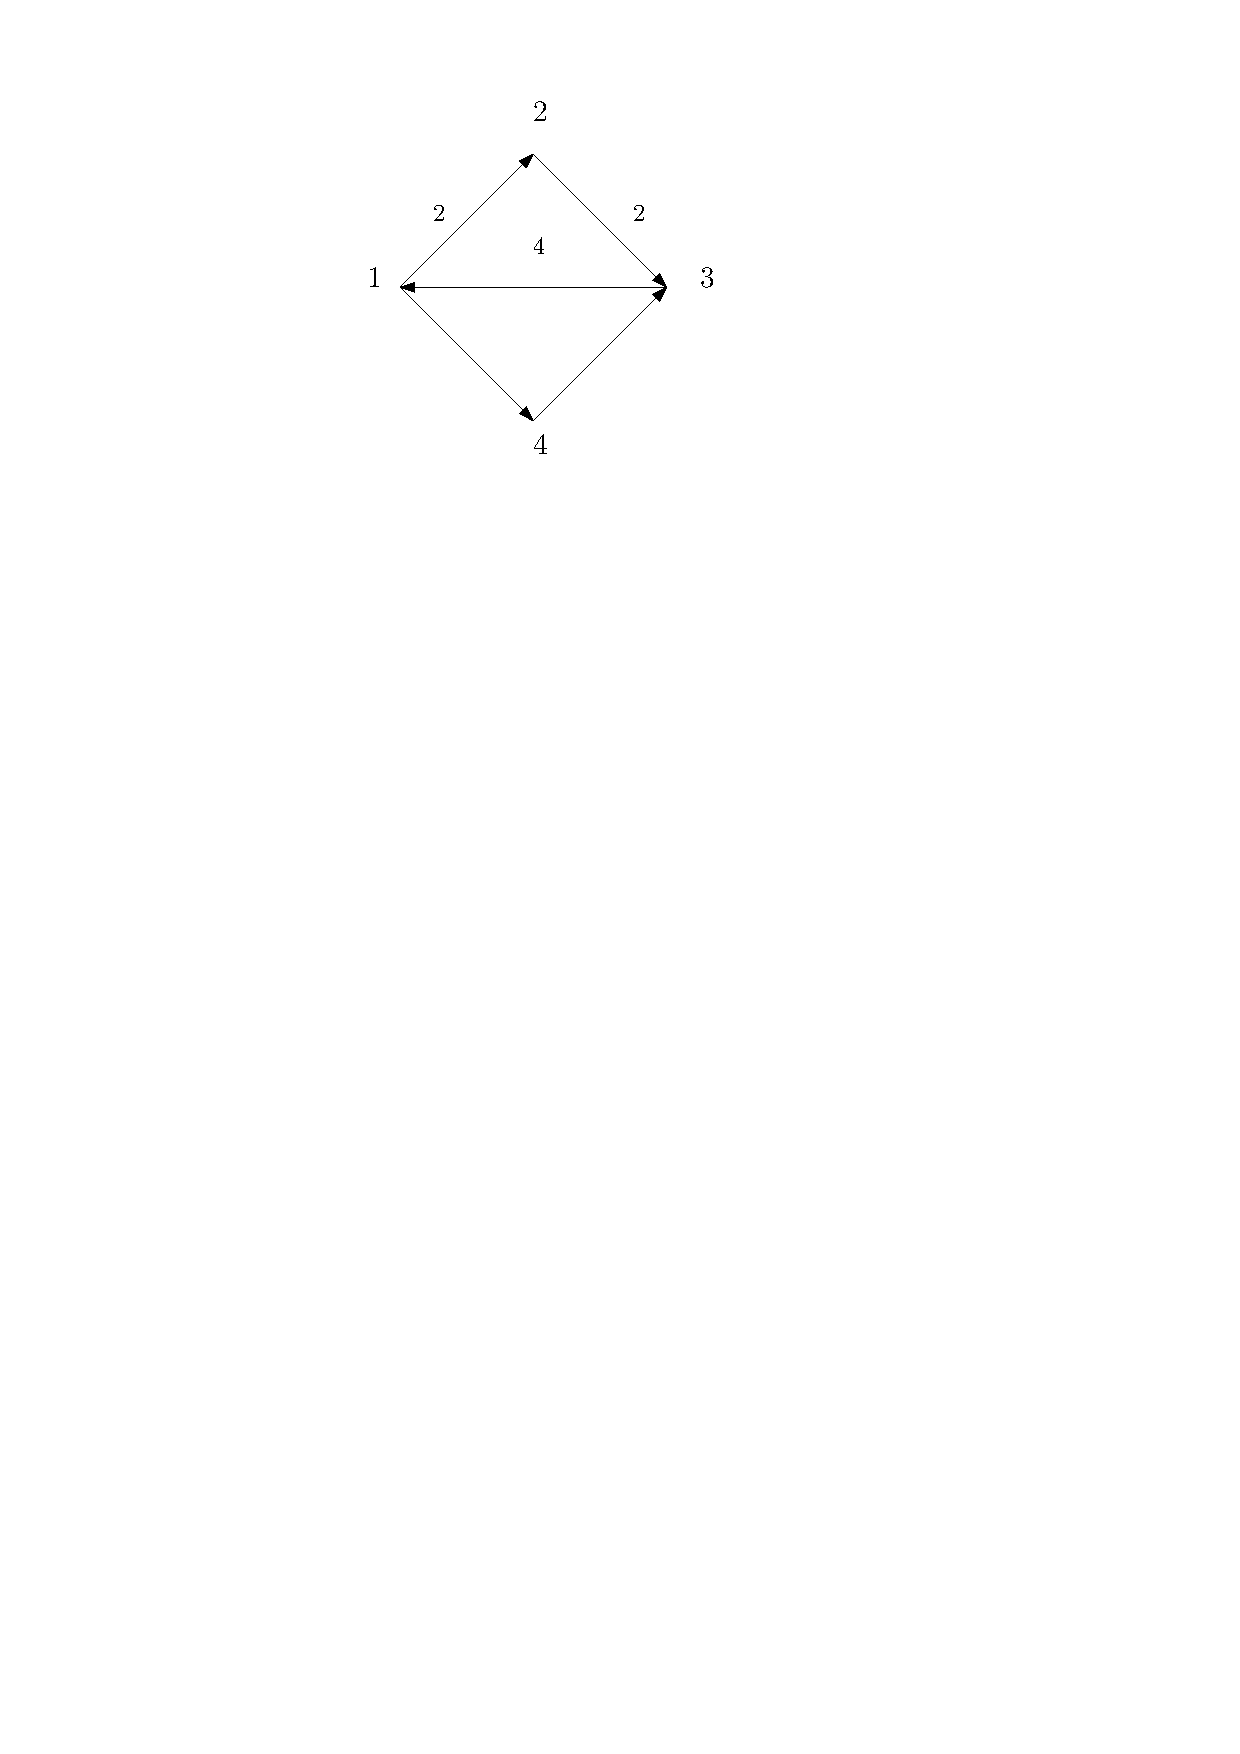
\includegraphics[scale = .50]{Diagram3.pdf}
\end{figure}
we add the relations $s_{2}s_{3}^{-1}(s_{4}s_{1}s_{4}^{-1})s_{3} = s_{3}^{-1}(s_{4}s_{1}s_{4}^{-1})s_{3}s_{2}$ and \\
$s_{2}s_{1}s_{4}^{-1}s_{3}s_{4}s_{1}^{-1} = s_{1}s_{4}^{-1}s_{3}s_{4}s_{1}^{-1}s_{2}$.
\end{frame}

\begin{frame}{Extending our Artin Group Presentations}
To a subdiagram of the form
\begin{figure}
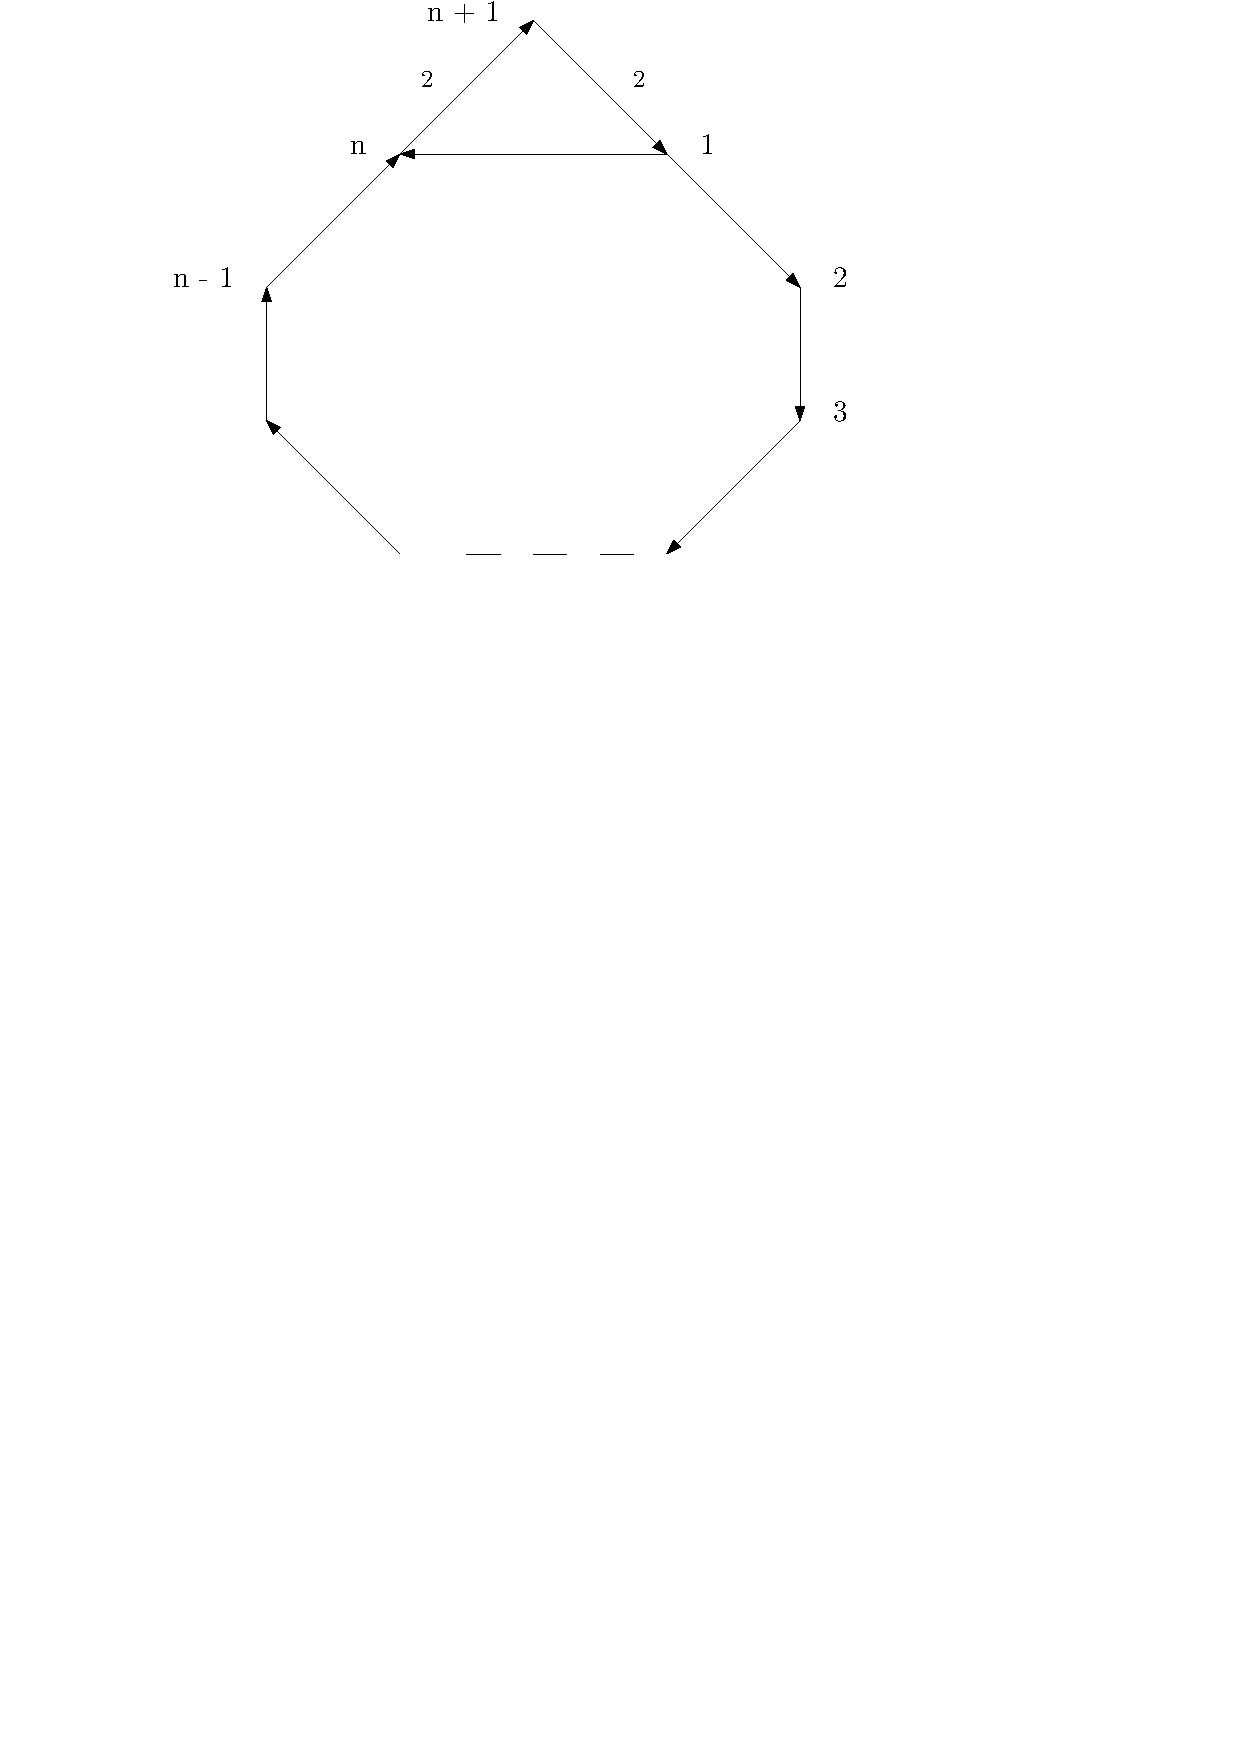
\includegraphics[scale = .50]{Diagram4.pdf}
\end{figure}
we add the relation $s_{1}(s_{2}^{-1} \dots s_{n-1}^{-1}(s_{n+1}s_{n}s_{n+1}^{-1})s_{n-1} \dots s_{2}) = (s_{2}^{-1} \dots s_{n-1}^{-1}(s_{n+1}s_{n}s_{n+1}^{-1})s_{n-1} \dots s_{2})s_{1}$.
\end{frame}

\begin{frame}{Extending our Artin Group Presentations}
To a subdiagram of the form
\begin{figure}
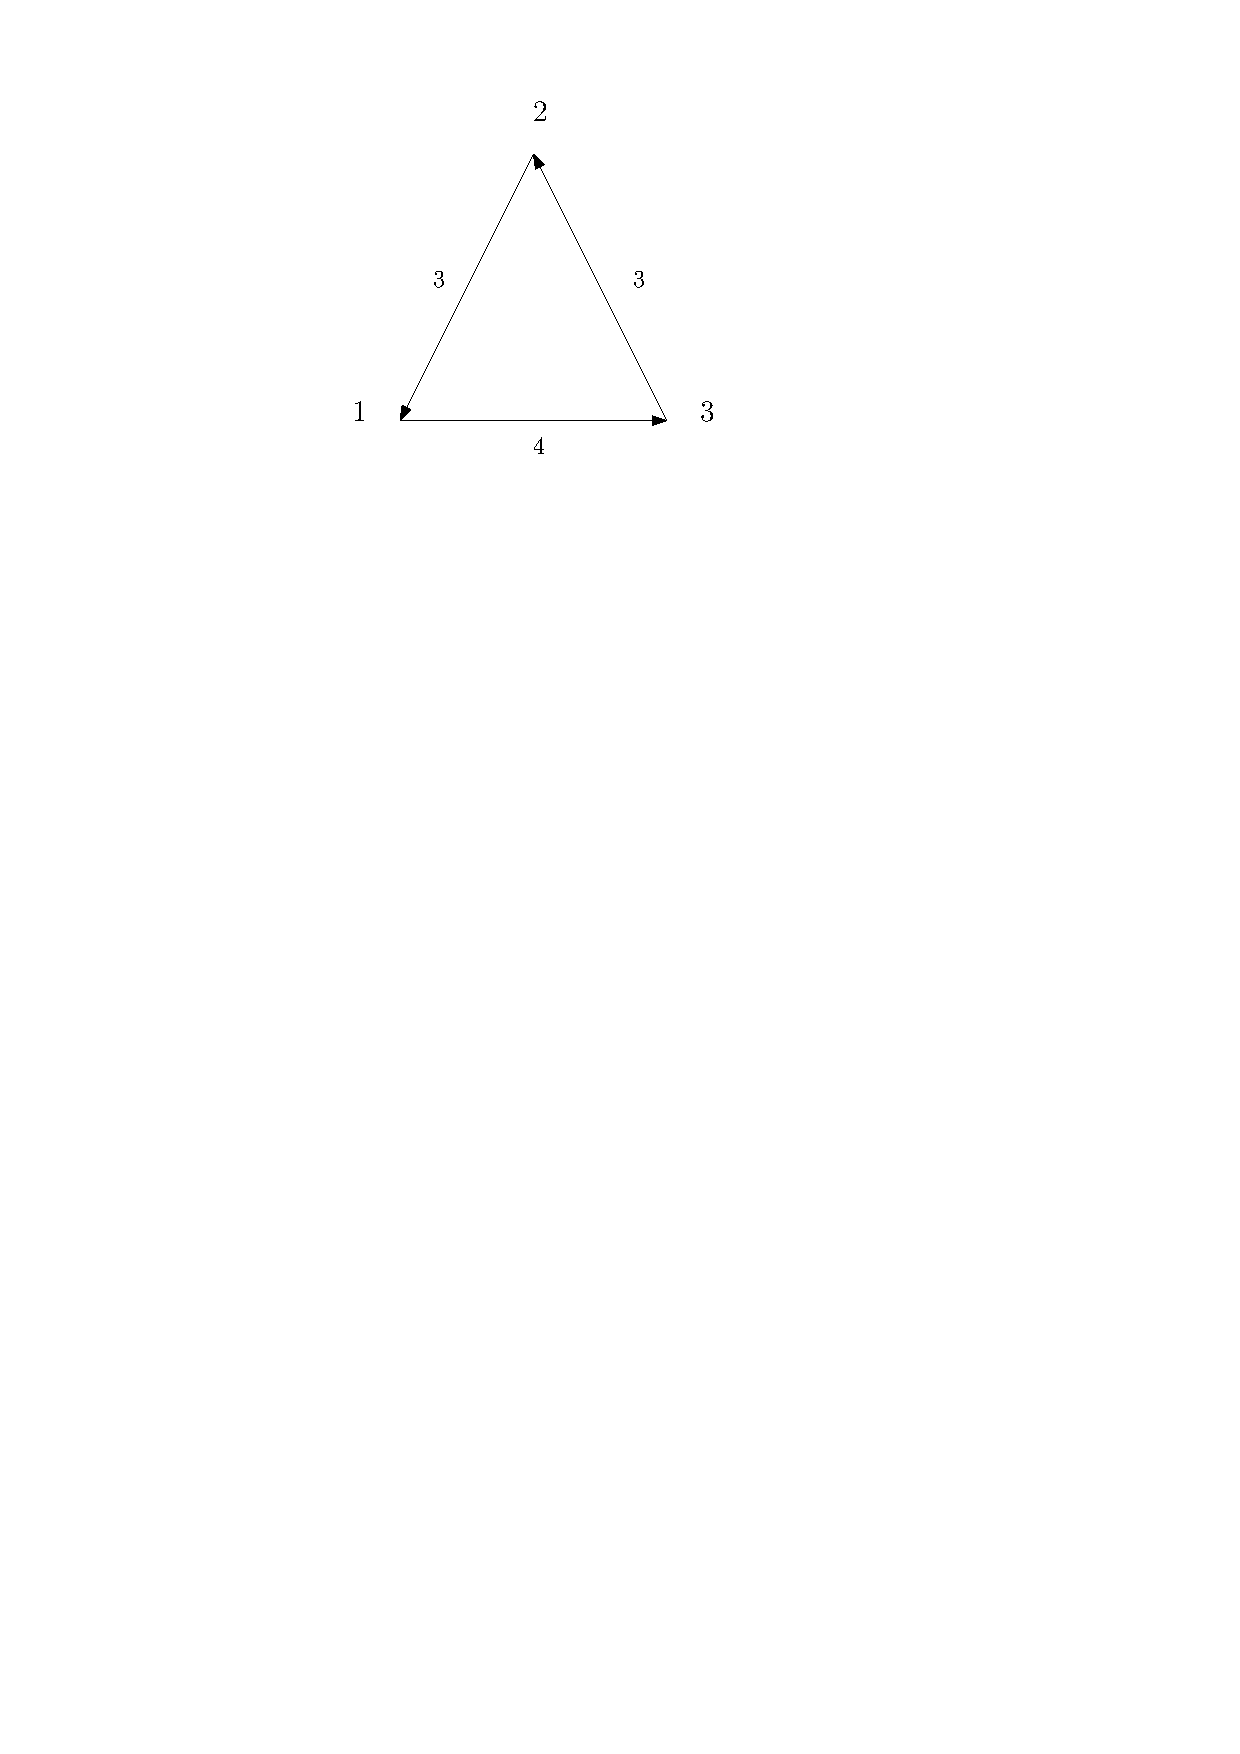
\includegraphics[scale = .50]{Diagram5.pdf}
\end{figure}
we add the relations $s_{2}s_{1}^{-1}(s_{2}s_{3}s_{2}^{-1})s_{1} = s_{1}^{-1}(s_{2}s_{3}s_{2}^{-1})s_{1}s_{2}$ and $s_{1}s_{2}s_{3}s_{2}s_{3}^{-1}s_{2}^{-1} = s_{2}s_{3}s_{2}s_{3}^{-1}s_{2}^{-1}s_{1}$.
\end{frame}

\begin{frame}
\begin{Conjecture}
$A_{\Gamma}$ is invariant up to isomorphism under diagram mutation.
\end{Conjecture}
\end{frame}








\begin{frame}
\begin{thebibliography}{69}

\bibitem{BM}[1] Barot, M. and Marsh, R., Reflection Group Presentations Arising from Cluster Algebras, \emph{Preprint}, arXiv:1112.2300 (2011)
\bibitem{FT}[2] Felikson, A. and Tumarkin, P., Coxeter groups and their quotients arising from cluster algebras, \emph{Preprint}, arXiv{1307.0672} (2013)
\bibitem{FZ}[3] Fomin, S. and Zelevinsky, A., Cluster Algebras I. Foundations, \emph{J. Amer. Math. Soc.}, \textbf{15} (2002), 497-529.
\bibitem{FZ}[4] Fomin, S. and Zelevinsky, A., Cluster Algebras II. Finite type classification, \emph{Invent. Math.}, \textbf{154} (2003), 63-121.

\end{thebibliography}

\end{frame}



\end{document}
